%\documentclass[12pt,a4paper]{report}
%\usepackage[utf8]{inputenc}
%\usepackage[francais]{babel}
%\usepackage[T1]{fontenc}
%\usepackage{amsmath}
%\usepackage{amsfonts}
%\usepackage{amssymb}
%\usepackage{float}
%\usepackage{graphicx}

%\author{Baptiste Lesquoy, Nicolas Weissenbach}
%\title{Expériences}

%\begin{document}
%\maketitle

\part{Matériel}

\chapter{Test du matériel}

\section{Objectif}
On voudrait savoir à quel point le matériel utilisé est fiable, et quelle précision on peut espérer avec.
On testera donc que la mousse qu'on compte utiliser pour rendre les micros plus unidirectionnel isole correctement, ainsi que l'effet de la mousse fournit de base avec les micros de plus on voudrait savoir jusqu'à quel degré les micros sont omnidirectionnels.
\section{Expérience}

\subsection{Configurations physique}
Dans chacune des expériences on gardera un micro témoin, le plus possible collé au micro servant de test (moins de 3cm à chaque fois) pour ne pas être influencé par autre chose. Seule exception: le test de la mousse incluse avec les micros, où on a procédé à un enregistrement avec et l'autre sans, sans changer le reste de la configuration.\\
Pour tester la mousse que l'on utilisera pour rendre les micros unidirectionnel, on enroule intégralement un micro dans cette mousse, l'autre micro est simplement posé à côté.\\
Pour tester les l'omnidirectionnalité, on positionne le micro témoin en face de l'émetteur, et un autre à côté, mais orienté de dos ou à 90 degrés de l'émetteur. Enfin on complétera en mettant les deux micros perpendiculaires à l'émetteur mais orienté vers des côtés opposés.

\subsection{Critères d'acceptation}
Pour la mousse, il est difficile de chiffrer le résultat, le but est juste de se donner une idée de son pouvoir isolant en visualisant des signaux lu avec et sans. Néanmoins, on s'attend à ce que: à partir d'un micro entouré de mousse, le signal ait une amplitude plus faible voir ait une forme globale différente d'un signal reçu sur un micro normal.\\
Pour les micros, on utilisera les deux configurations où les micros sont tous les deux de face pour savoir s'il existe des différences entre les deux au niveau de l'amplitude du signal reçu, voir si on constate un décalage de phase (même minime), et si possible chiffrer ces différences. On voudrait aussi savoir à quel point ils sont omnidirectionnel et quantifier les différences entre les signaux reçus selon l'orientation du micro par rapport à la source.


\subsection{Signal émis}
On a utilisé le signal carré de 5 échantillons(voir \ref{signal_carre}) afin de repérer facilement les signaux venant de l'émetteur.

\subsection{Réception du signal}
On utilise le montage habituel (voir \ref{protocole}).

\section{Résultats}

\subsection{Entre les deux micros}\label{differences_entre_micros}

\begin{figure}[H]
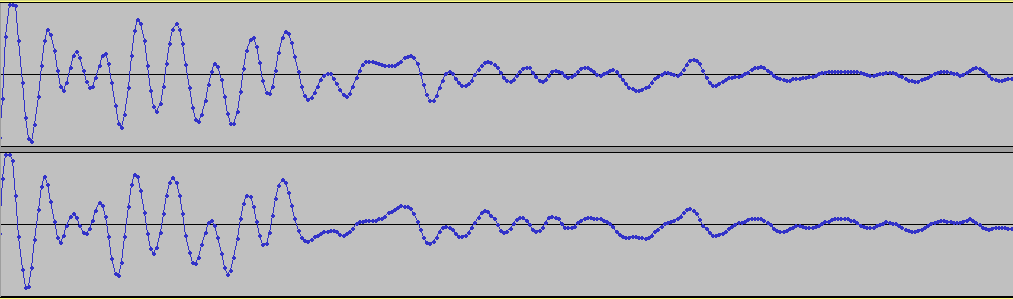
\includegraphics[width=\textwidth]{resources/img/micros_face.png}
\caption{signaux des deux micros côte à côte}
\end{figure}
On ne constate pas de grosses différences entre les deux micros. la forme globale du signal capté est la même, il y a parfois quelques irrégularités, mais elle ne sont ni importantes, ni très fréquentes. L'amplitude est sensiblement identique et on ne constate aucun décalage de phase.

\subsection{mousse de base des micros}

\begin{figure}[H]
\begin{tabular}{ll}
 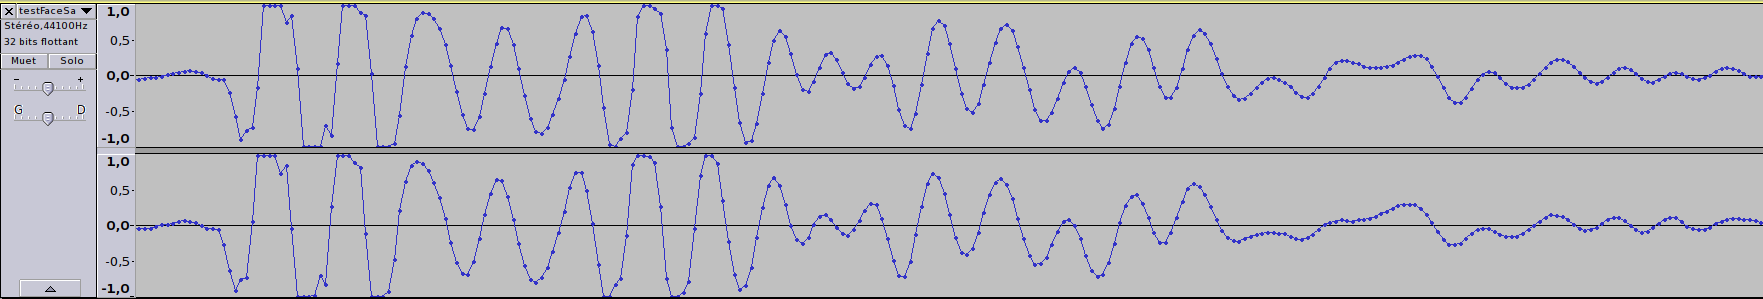
\includegraphics[scale=0.15]{resources/img/signal_sans_mousse.png}
&  
 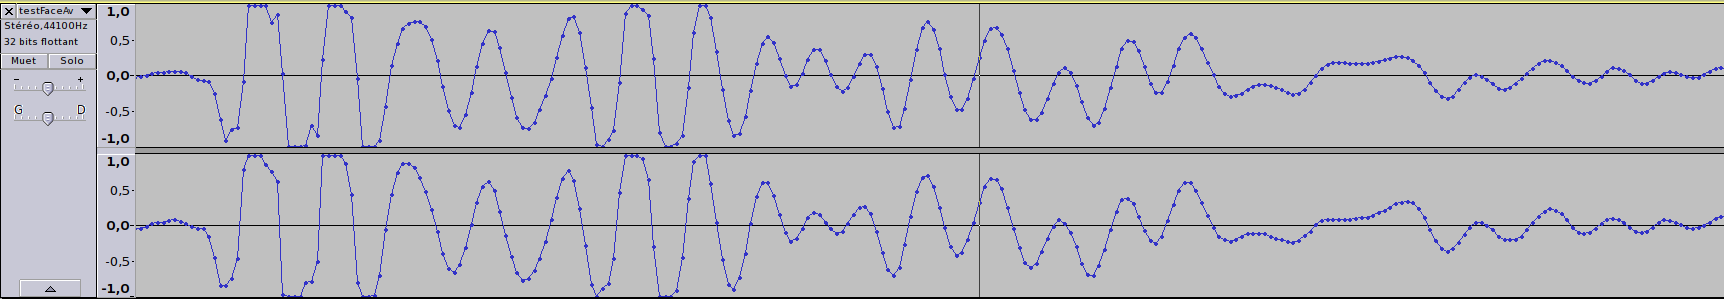
\includegraphics[scale=0.15]{resources/img/signal_avec_mousse.png}
 \\
\end{tabular}
\caption{à gauche le signal sans mousse, à droite avec}
\end{figure}
On ne remarque pas vraiment de différence entre les deux, la mousse de base semble donc peu utile.

\subsection{mousse isolante}
\begin{figure}[H]
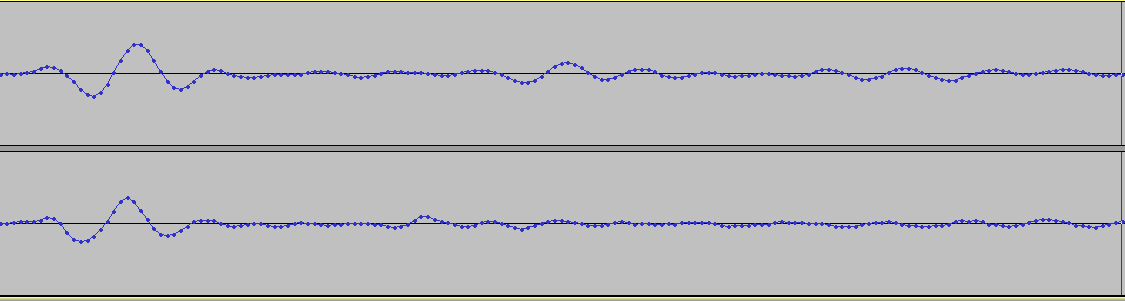
\includegraphics[width=\textwidth]{resources/img/isolation.png}
\caption{en haut le micro sans isolation, en bas celui avec}
\end{figure}
On constate que la mousse isolante atténue bien l'amplitude du signal reçu. Il y a un léger décalage de phase (de 1 à 3 échantillons selon ce que l'on mesure), néanmoins on ne peut rien en conclure car la position et l'orientation précise du micro dans la mousse est inconnue. Par contre on remarque que le signal qui suit l'impulsion est assez différent sur les deux, cette partie du signal correspondant à l'écho, on peut en déduire que celui-ci est partiellement filtré par la mousse isolante.

\subsection{Orientation des micros}
\label{orientation_micro}
\subsubsection{Un micro perpendiculaire à l'émetteur}
\begin{figure}[H]
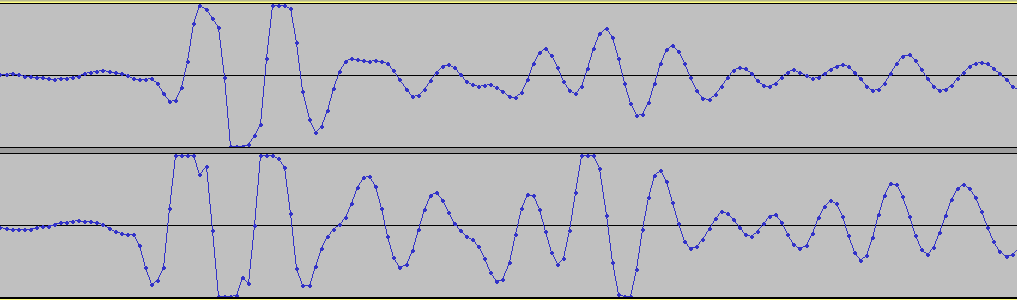
\includegraphics[width=\textwidth]{resources/img/90.png}
\caption{en haut le micro de référence, en bas celui orienté à 90 degrés de l'émetteur}
\end{figure}
On constate que la différence d'amplitude est grandes entre les deux signaux. De plus il y a un décalage de phase: il est de 3 à 4 échantillons au début du signal et de 1 à 2 échantillons dans l'écho.
Enfin on remarque que les deux signaux peuvent différer à certains endroits (notamment dans le début de l'écho).

\subsubsection{Deux micros perpendiculaires à l'émetteur(dos à dos)}
\begin{figure}[H]
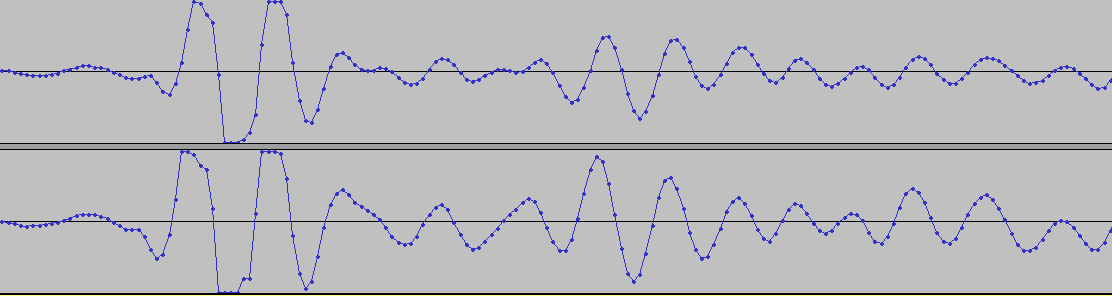
\includegraphics[width=\textwidth]{resources/img/dos_a_dos.png}
\caption{signaux reçus quand les micros sont dos à dos}
\end{figure}
Dos à dos on retrouve des signaux plus identiques l'un à l'autre que lorsque seul un des deux est perpendiculaire à la source. L'amplitude est la même pour les deux signaux, et le décalage de phase est de 1 à 2 échantillons pour le tout début de l'impulsion puis de 0 à 1 échantillons dans l'écho. On remarques quelques différences, mais pas plus que ce qui est normal(voir \ref{differences_entre_micros}).

\subsubsection{Dos à l'émetteur}
\begin{figure}[H]
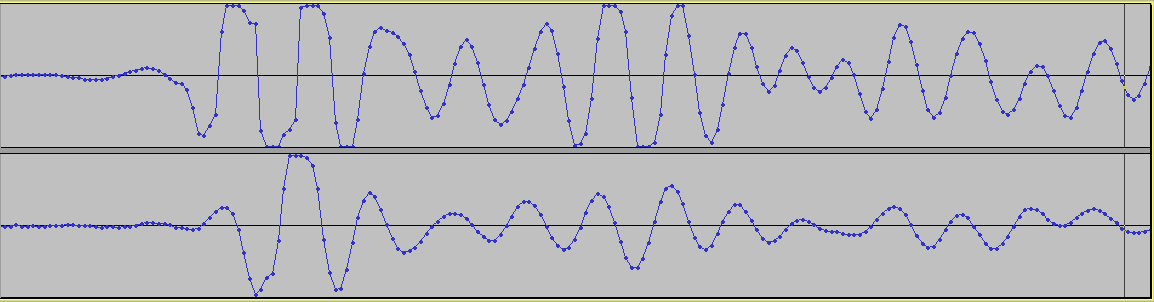
\includegraphics[width=\textwidth]{resources/img/dos_a_la_source.png}
\caption{en haut le témoin, en bas le micro dos à l'émetteur}
\end{figure}
Les signaux reçus sont très différents, la seule partie que l'on peut identifier clairement étant le tout début de l'impulsion. Sur cette dernière on constate un écart de phase de 11 échantillons.

\section{Conclusion}
De toutes ces expériences on peut en déduire:
\begin{itemize}
\item les micros sont fiables et il n'y a pas de différences notables entre les deux.
\item la mousse de base semble inutile
\item la mousse isolante réduit assez clairement l'amplitude du signal capté, hypothétiquement on peut s'en servir pour réduire l'écho.
\item il y a des différences dans les signaux reçus en fonction de l'orientation du micro. si un des micros est dos à l'émetteur alors que l'autre est de face, le signal en devient même impossible à reconnaitre. Si on reste dans une disposition avec un micro à 90 degrés de l'émetteur l'écart est très faible, et s'annule quasiment si le deuxième aussi est à 90 degrés(dans le sens inverse). On peut donc conjecturer que tant qu'on reste dans une orientation de moins de 90 degrés le signal reste exploitable.
\end{itemize}





\chapter{Élaboration du protocole}
\section{Objectif}
On aimerait définir un protocole qui permettrait de mesurer précisément un décalage de phase sur un signal enregistré en même temps par deux micros différents.


\section{Expérience}
\subsection{Critères d'acceptation}
On considérera que le protocole est bon si on arrive systématiquement et dans plusieurs configurations à retrouver les distances physiques séparant l'émetteur du signal de chacun des micros. De plus on vérifiera que le décalage de phase entre les micros correspond bien à la distance les séparant.

\subsection{Configurations}
Tout au long du document, on utilisera les termes m1 et m2 pour désigner les deux micros, x l'espace entre les micros, s1 la source sonore (le haut-parleur), et y la distance entre m2 et s1. De sorte que la configuration avec les micros et le haut-parleur aligné puisse être schématisé comme si dessous:
\begin{figure}[H]
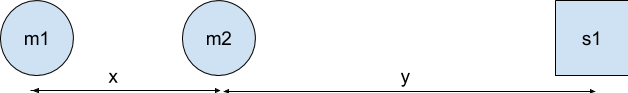
\includegraphics[width=\textwidth]{../tests/test_du_protocole/schema.png} 
\caption{Schéma de l'expérience avec les micros et le haut-parleur alignés}
\end{figure}
les différentes configurations choisies sont:
\begin{itemize}
\item m1, m2 et s1 sont alignés, on teste différentes valeurs de x et y.
\item m1 et m2 sont côte à côte, plus ou moins collés.
\end{itemize}
\subsection{Signal émis}
On utilisera un fichier sonore wav qui:
\begin{itemize}
\item dure 3 secondes
\item est un sinus à une fréquence constante a 300Hz
\item a un taux d'échantillonnage de 44100Hz
\item est un fichier mono
\end{itemize}
Le signal est émis depuis une enceinte branché à un ordinateur via une prise jack 3.5.



\subsection{Réception du signal}
Le signal est enregistré via deux micros identiques (même modèle), posés sur de la mousse. Le tout est coordonné par un contrôleur trik sur lequel les micros sont branchés via deux prises jack 3.5 séparées.
On enregistre le signal réceptionné dans un fichier wav avec un taux d'échantillonnage de 44100Hz.
Chaque enregistrement dur 6 secondes, on commence par démarrer l'enregistrement, puis on attend une à 2 secondes avant d'émettre le signal. Ainsi on peut observer le bruit ambiant et être sûr de capter l'intégralité du signal émis.
Les calculs de distances et de décalage de phase seront fait par rapport aux premiers échantillons reçus du signal, afin de ne pas être influencé par l'écho.

\section{Résultats/conclusions}
\subsection{Tout aligné}
\begin{figure}[H]
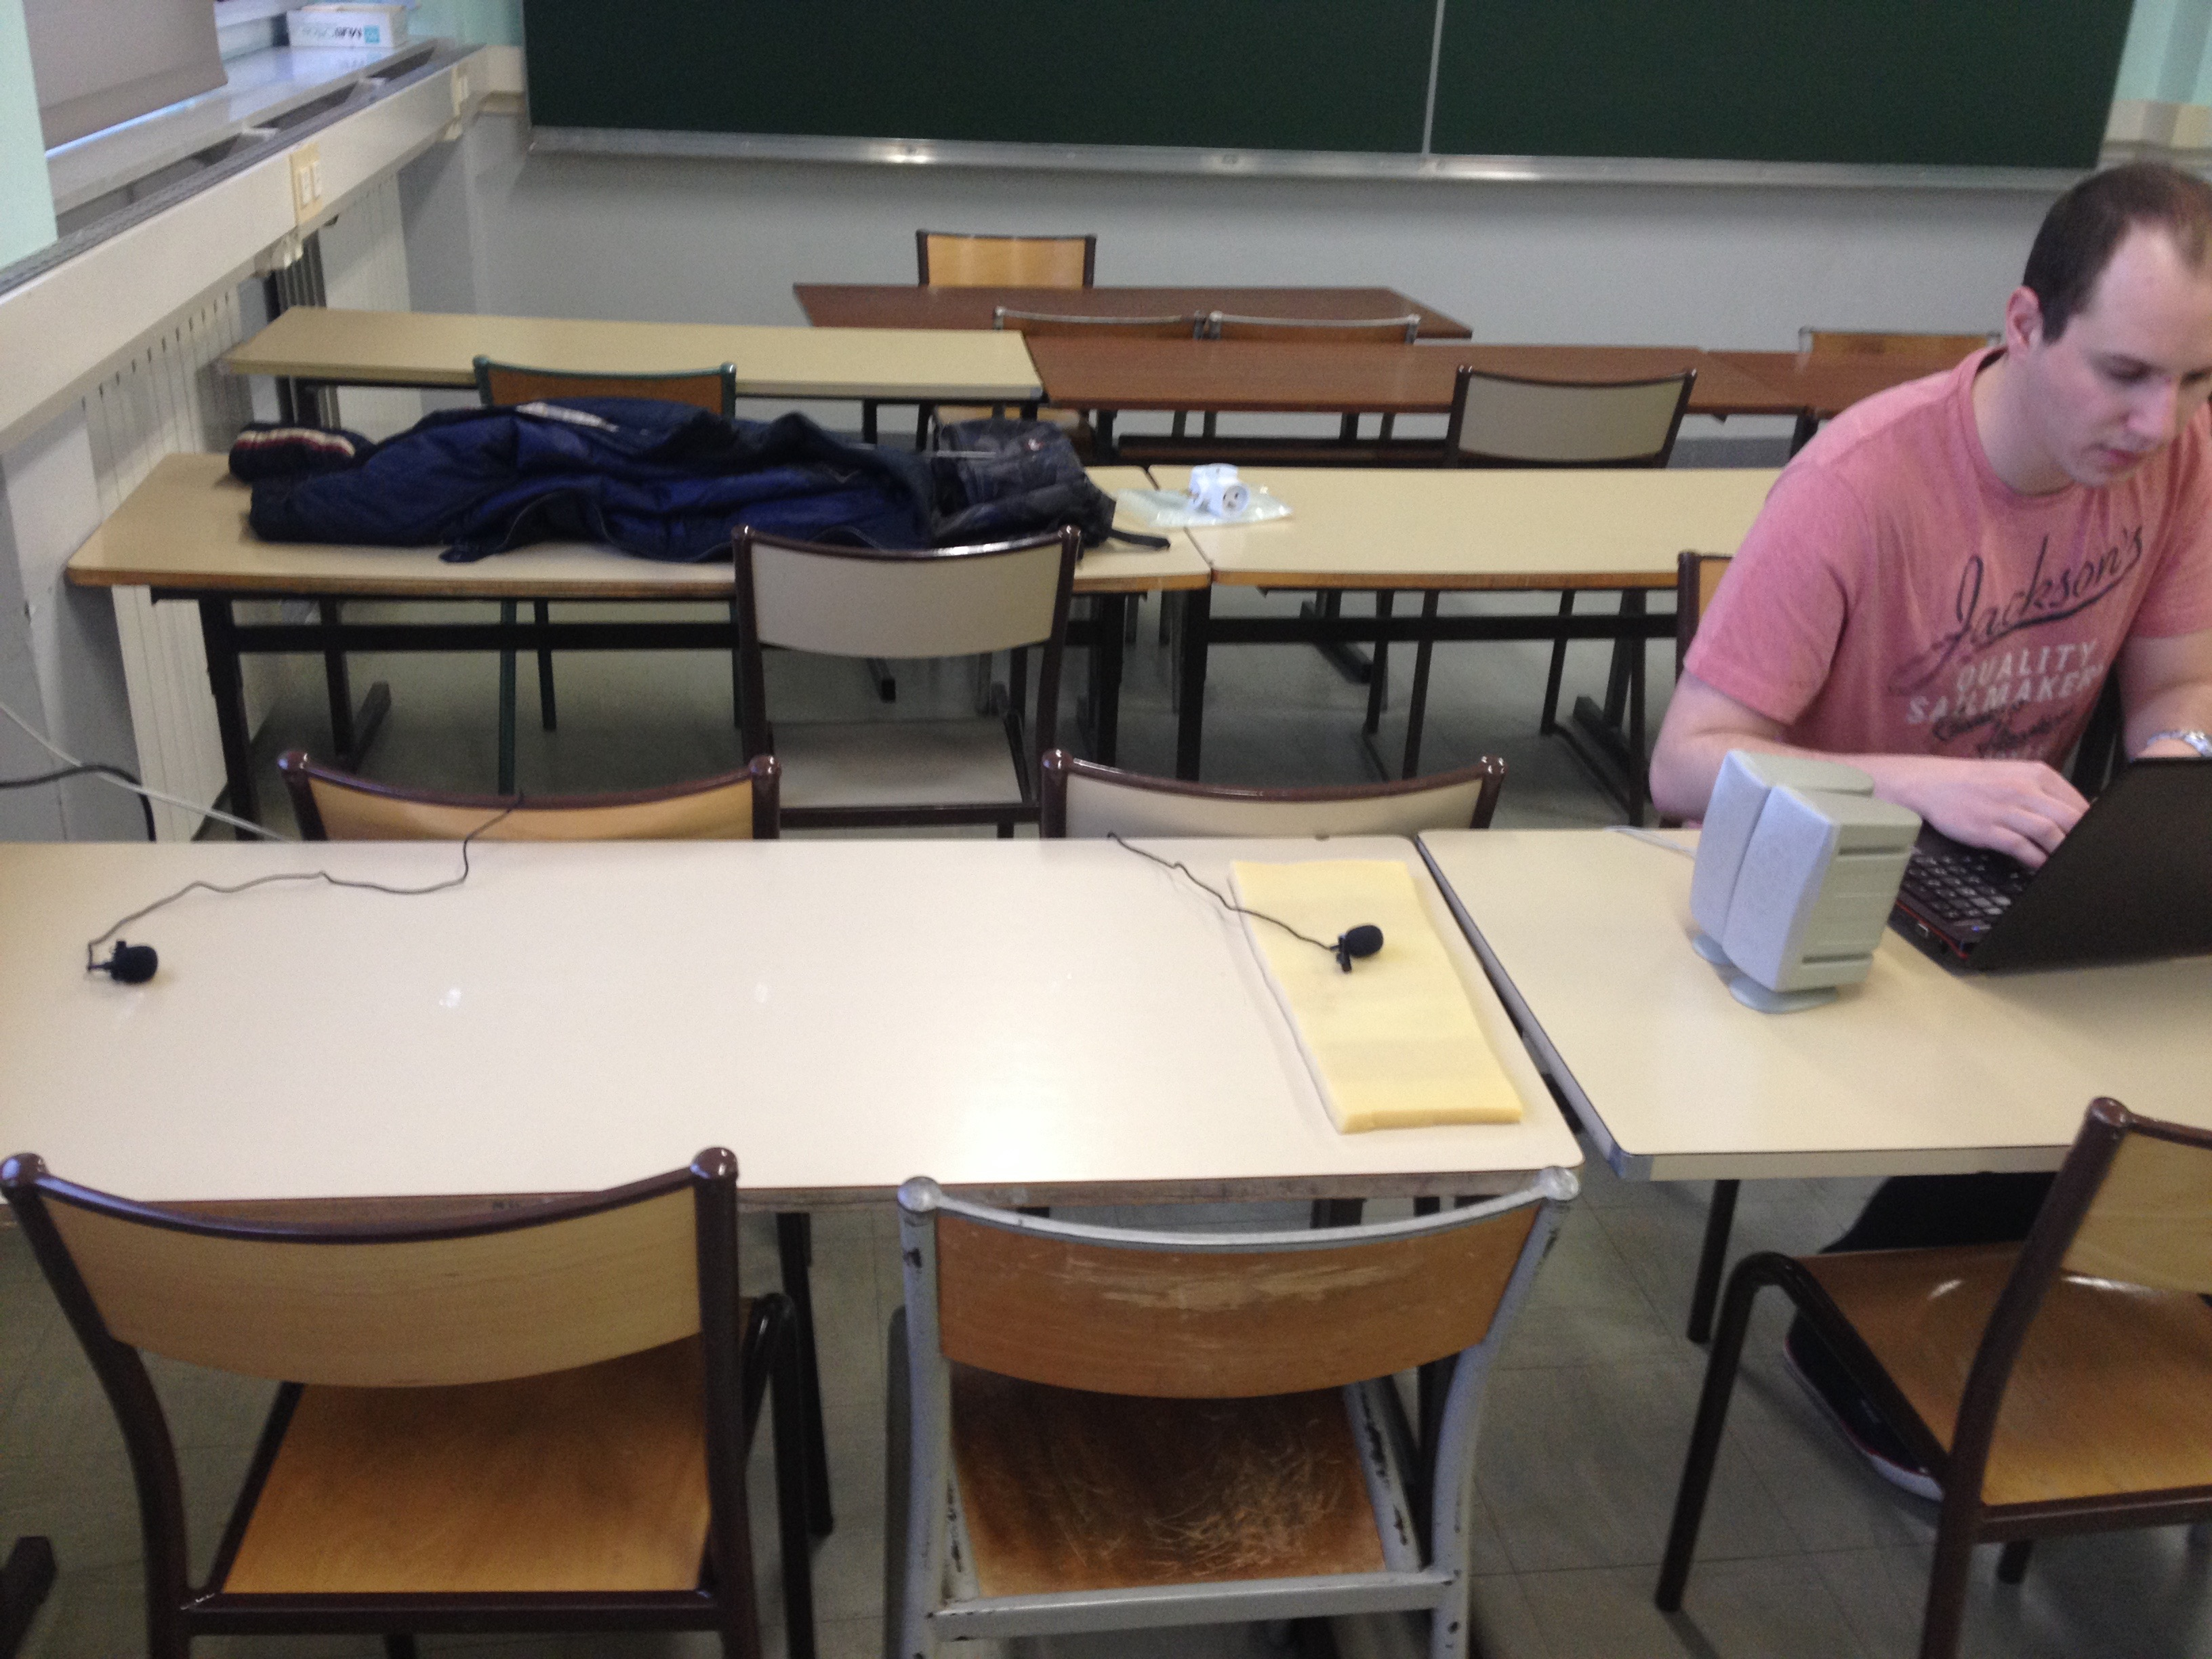
\includegraphics[width=\textwidth]{../tests/test_du_protocole/micros_alignes.jpg} 
\caption{expérience avec les micros et l'enceinte aligné}
\end{figure}


\begin{figure}[H]
\begin{tabular}{|l || p{1.5cm} | p{1.5cm} | p{1.5cm} | p{1.5cm} | p{1.5cm} | p{1.5cm} | p{1.5cm}  |}
\hline
\# & $f$ (Hz) & $x$ (mm) & $y$ (mm) & durée (s) & décalage de phase (échantillons) & décalage de phase (s) & décalage de phase (m)\\
\hline
\hline
1	& 80 & 220 &	500&	3&	266&	0.0014&	0.476\\
2	&80	&220	&500	&3	&287	&0.0015&	0.51\\
3	&80	&220	&500	&3	&273	&0.0014	&0.476\\
4	&80	&220	&500	&3	&281	&0.0015	&0.51\\
5	&80	&220	&500	&3	&273	&0.0014	&0.476\\
6	&80	&220	&500	&3	&271	&0.0014	&0.476\\
7	&80	&220	&500	&3	&269	&0.0014	&0.476\\
8	&80	&220	&500	&3	&284	&0.0015	&0.51\\
9	&80	&220	&500	&3	&282	&0.0015	&0.51\\
10&	80&	220	&500	&3	&272	&0.0014	&0.476\\
\hline
11&	80&	500	&260	&3	&923	&0.0048	&1.632\\
12&	80&	500	&260	&3	&844	&0.0044	&1.496\\
13&	80&	500	&260	&3	&836	&0.0044	&1.496\\
14&	80&	500	&260	&3	&836	&0.0044	&1.496\\
15&	80&	500	&260	&3	&845	&0.0044	&1.496\\
16&	80&	500	&260	&3	&915	&0.0048	&1.632\\
17&	80&	500	&260	&3	&852	&0.0044	&1.496\\
18&	80&	500	&260	&3	&850	&0.0044	&1.496\\
19&	80&	500	&260	&3	&844	&0.0044	&1.496\\
20&	80&	500	&260	&3	&849	&0.0044	&1.496\\
\hline
\end{tabular}
où : 
\begin{description}
\item[$f$] est la fréquence utilisé.
\item[$x$] est la distance entre la source sonore et le premier micro
\item[$y$] est la distance entre les deux micros
\end{description}
\caption{tableau des résultats de toutes les itération de l'expérience avec les micros et enceintes alignés}
\end{figure}


\subsection{Récepteurs côte à côte}
\begin{figure}[H]
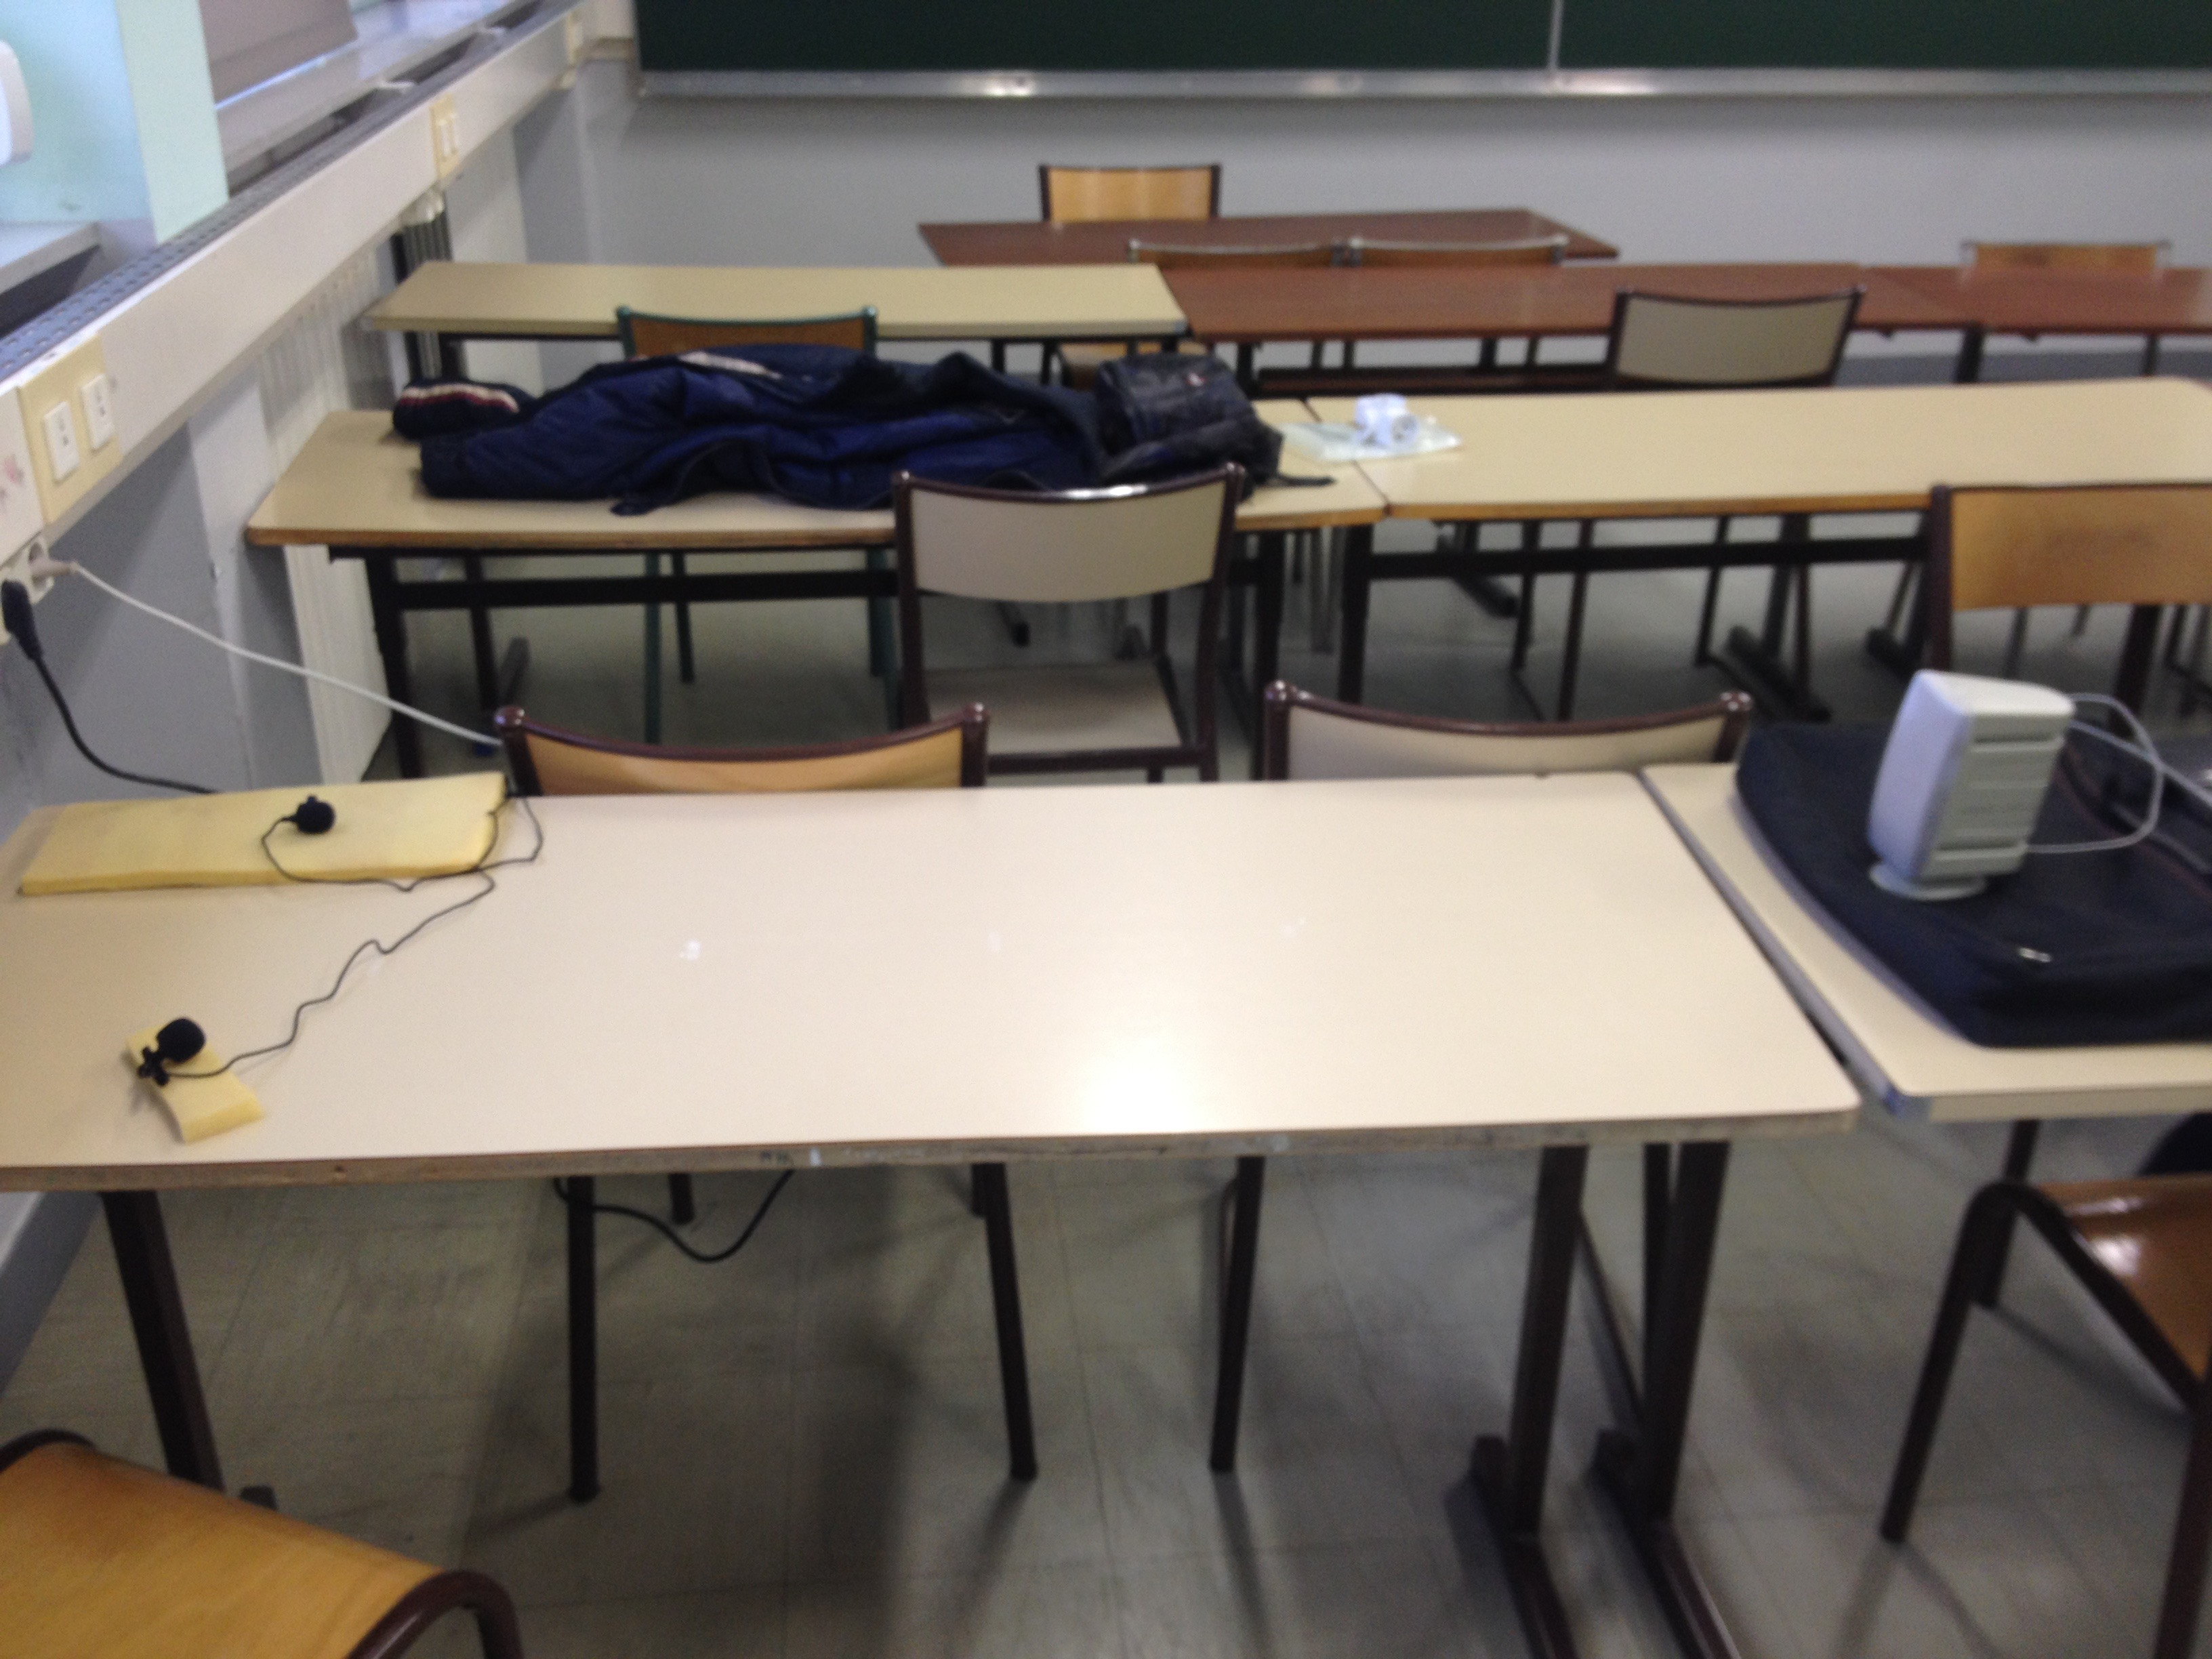
\includegraphics[width=\textwidth]{../tests/test_du_protocole/micros_cote_a_cote.jpg} 
\end{figure}

\begin{figure}[H]
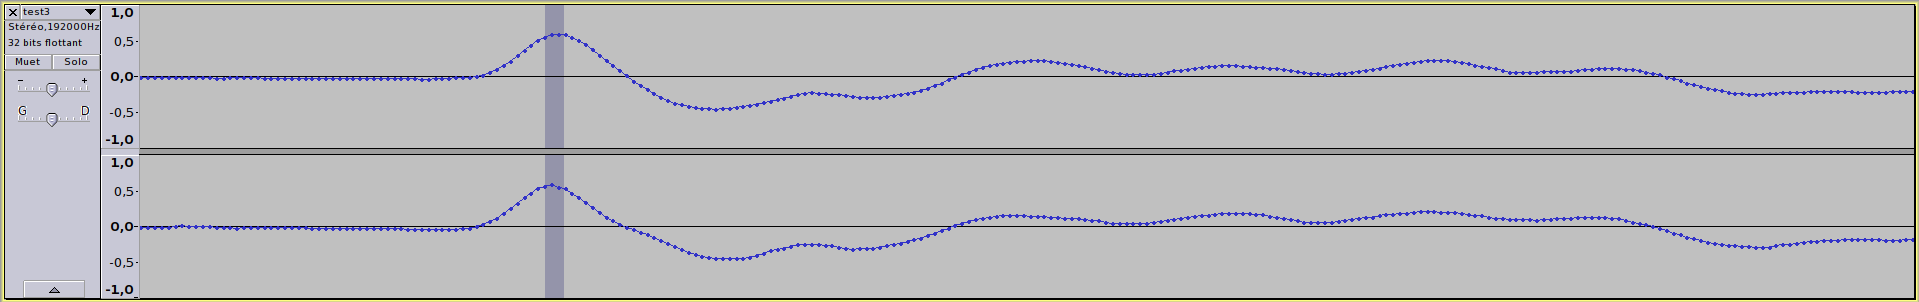
\includegraphics[width=\textwidth]{../tests/test_du_protocole/mesures_micro_colles/colles.png} 
\caption{signaux reçu par les deux micros lorsqu'ils sont collés}
\end{figure}

\begin{figure}[H]
\begin{tabular}{|l || p{1.4cm} | p{1.4cm} | p{1.4cm} | p{1.4cm} | p{1.4cm} | p{1.7cm} | p{1.7cm}  |}
\hline
\# & $f$ (Hz) & $x$ (mm) & $y$ (mm) & durée (s) & décalage de phase (échantillons) & décalage de phase (s) & décalage de phase (m)\\
\hline
\hline
1	&80	&220	&500	&3	&2	&0.0000104	&0.003536\\
2	&80	&220	&500	&3	&2	&0.0000104	&0.003536\\
3	&80	&220	&500	&3	&1	&0.0000052	&0.001768\\
\hline
\end{tabular}
où : 
\begin{description}
\item[$f$] est la fréquence utilisé.
\item[$x$] est la distance entre la source sonore et le premier micro
\item[$y$] est la distance entre les deux micros
\end{description}
\caption{tableau des résultats de toutes les itération de l'expérience avec les micros collé}
\end{figure}

On constate bien qu'il n'y a pas de décalage quand les deux micros sont collés. Par contre on remarque une différence d'intensité, qui peut être expliqué par une simple différence du matériel. Les micros n'étant pas des micros professionnels, ce n'est pas étonnant que la qualité ne soit pas constante d'un micro à l'autre.


\chapter{Décalage de phase}
\section{Objectif}
Dans l'expérience précédente on a ignoré l'écho, cette fois si, on aimerait savoir à quel point l'écho peut avoir de l'importance dans le signal reçu, et plus particulièrement dans le décalage de phase entre les deux micro .
On va donc utiliser de la mousse pour rendre les micros plus "directionnels" et regarder si ça a de l'influence sur les données enregistrées selon la direction donné.

\section{Expérience}
\subsection{Critères d'acceptation}
On commencera par reprendre la dernière configuration de l'expérience précédente en ajoutant un cône autour d'un des micros afin de vérifier que le signal reçu est différent avec et sans le cône (donc que la mousse est bien efficace pour filtrer le signal).
On considérera que l'écho a de l'influence sur le signal reçu si en changeant l'orientation d'un micro placé dans un cône en mousse on observe un décalage de phase par rapport à un micro sans cône (donc omnidirectionnel).

\subsection{Configurations}
On reprend la configuration précédente. Cette fois, on placera les micros côte à côte et on changera uniquement l'orientation  du micro entouré d'un cône de mousse.

\subsection{Signal émis et réception}
Le matériel et les paramètres sont les mêmes que pour l'expérience précédente à la seule différence du cône en mousse autour d'un des micros.

\section{Résultats/conclusions}


\subsection{Vérification de l'efficacité de la mousse}
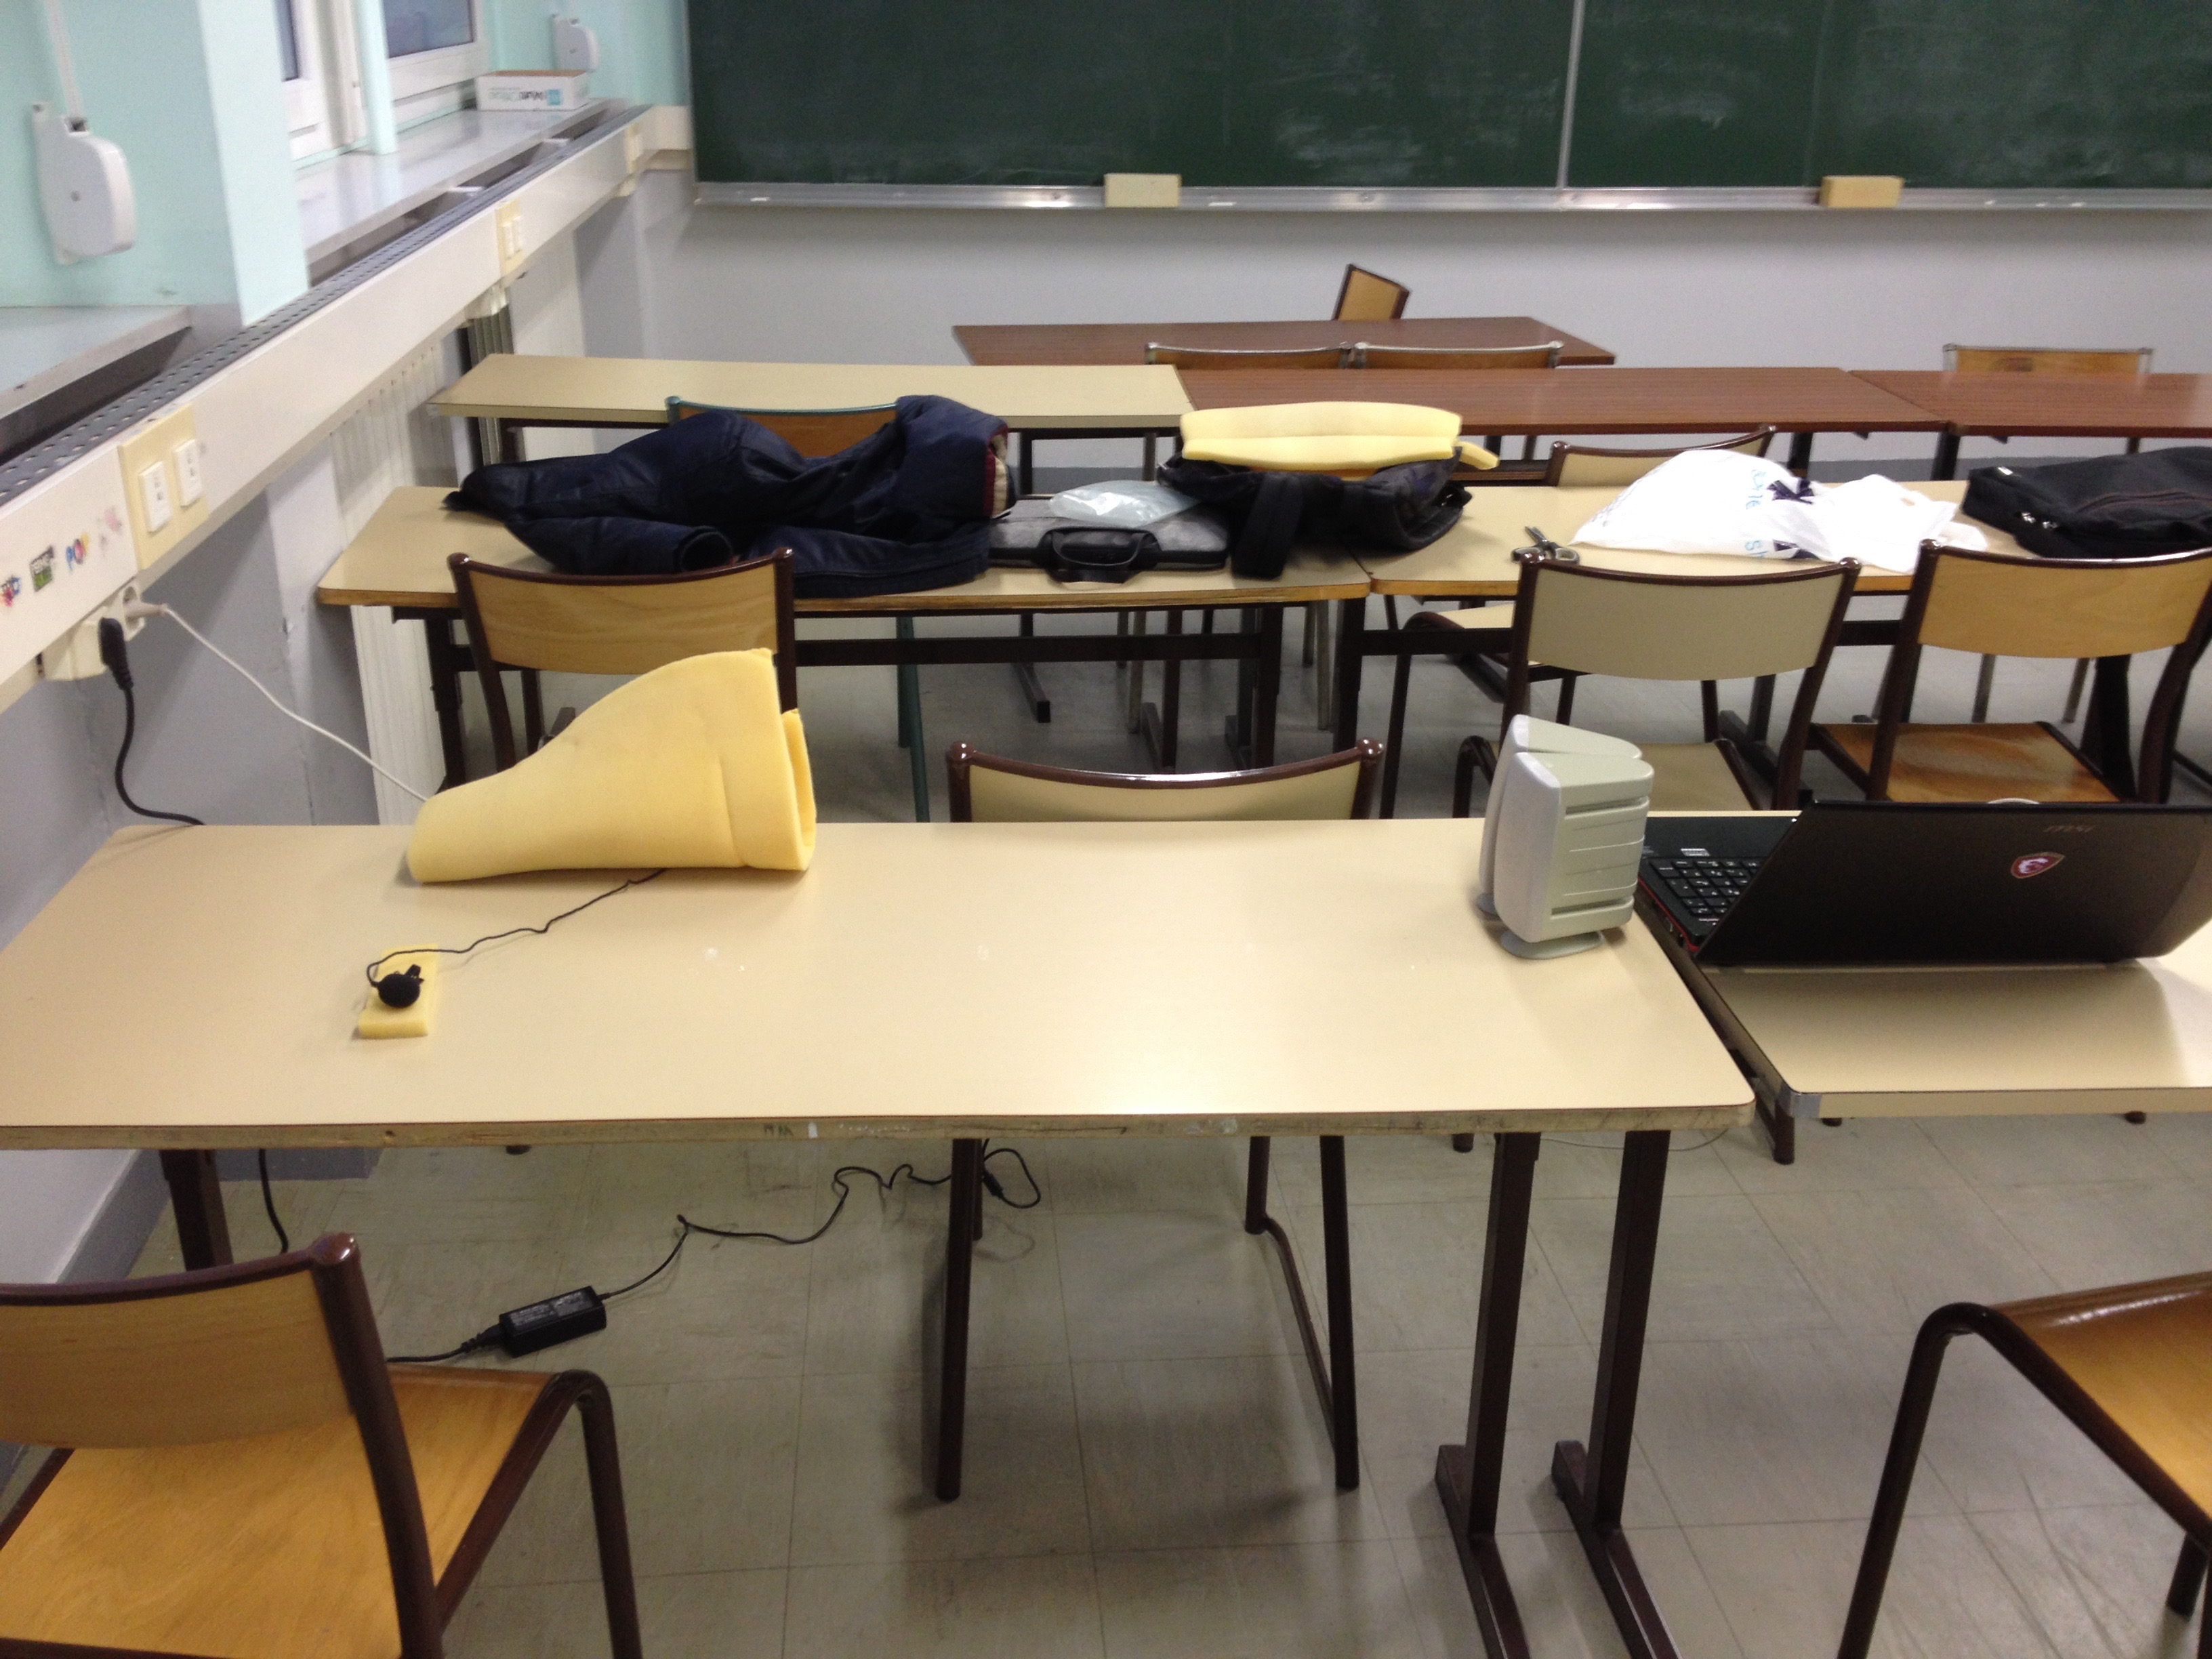
\includegraphics[width=\textwidth]{../tests/test_du_protocole/cone_face.jpg} 

\subsection{Changement d'orientation}


\begin{figure}[H]
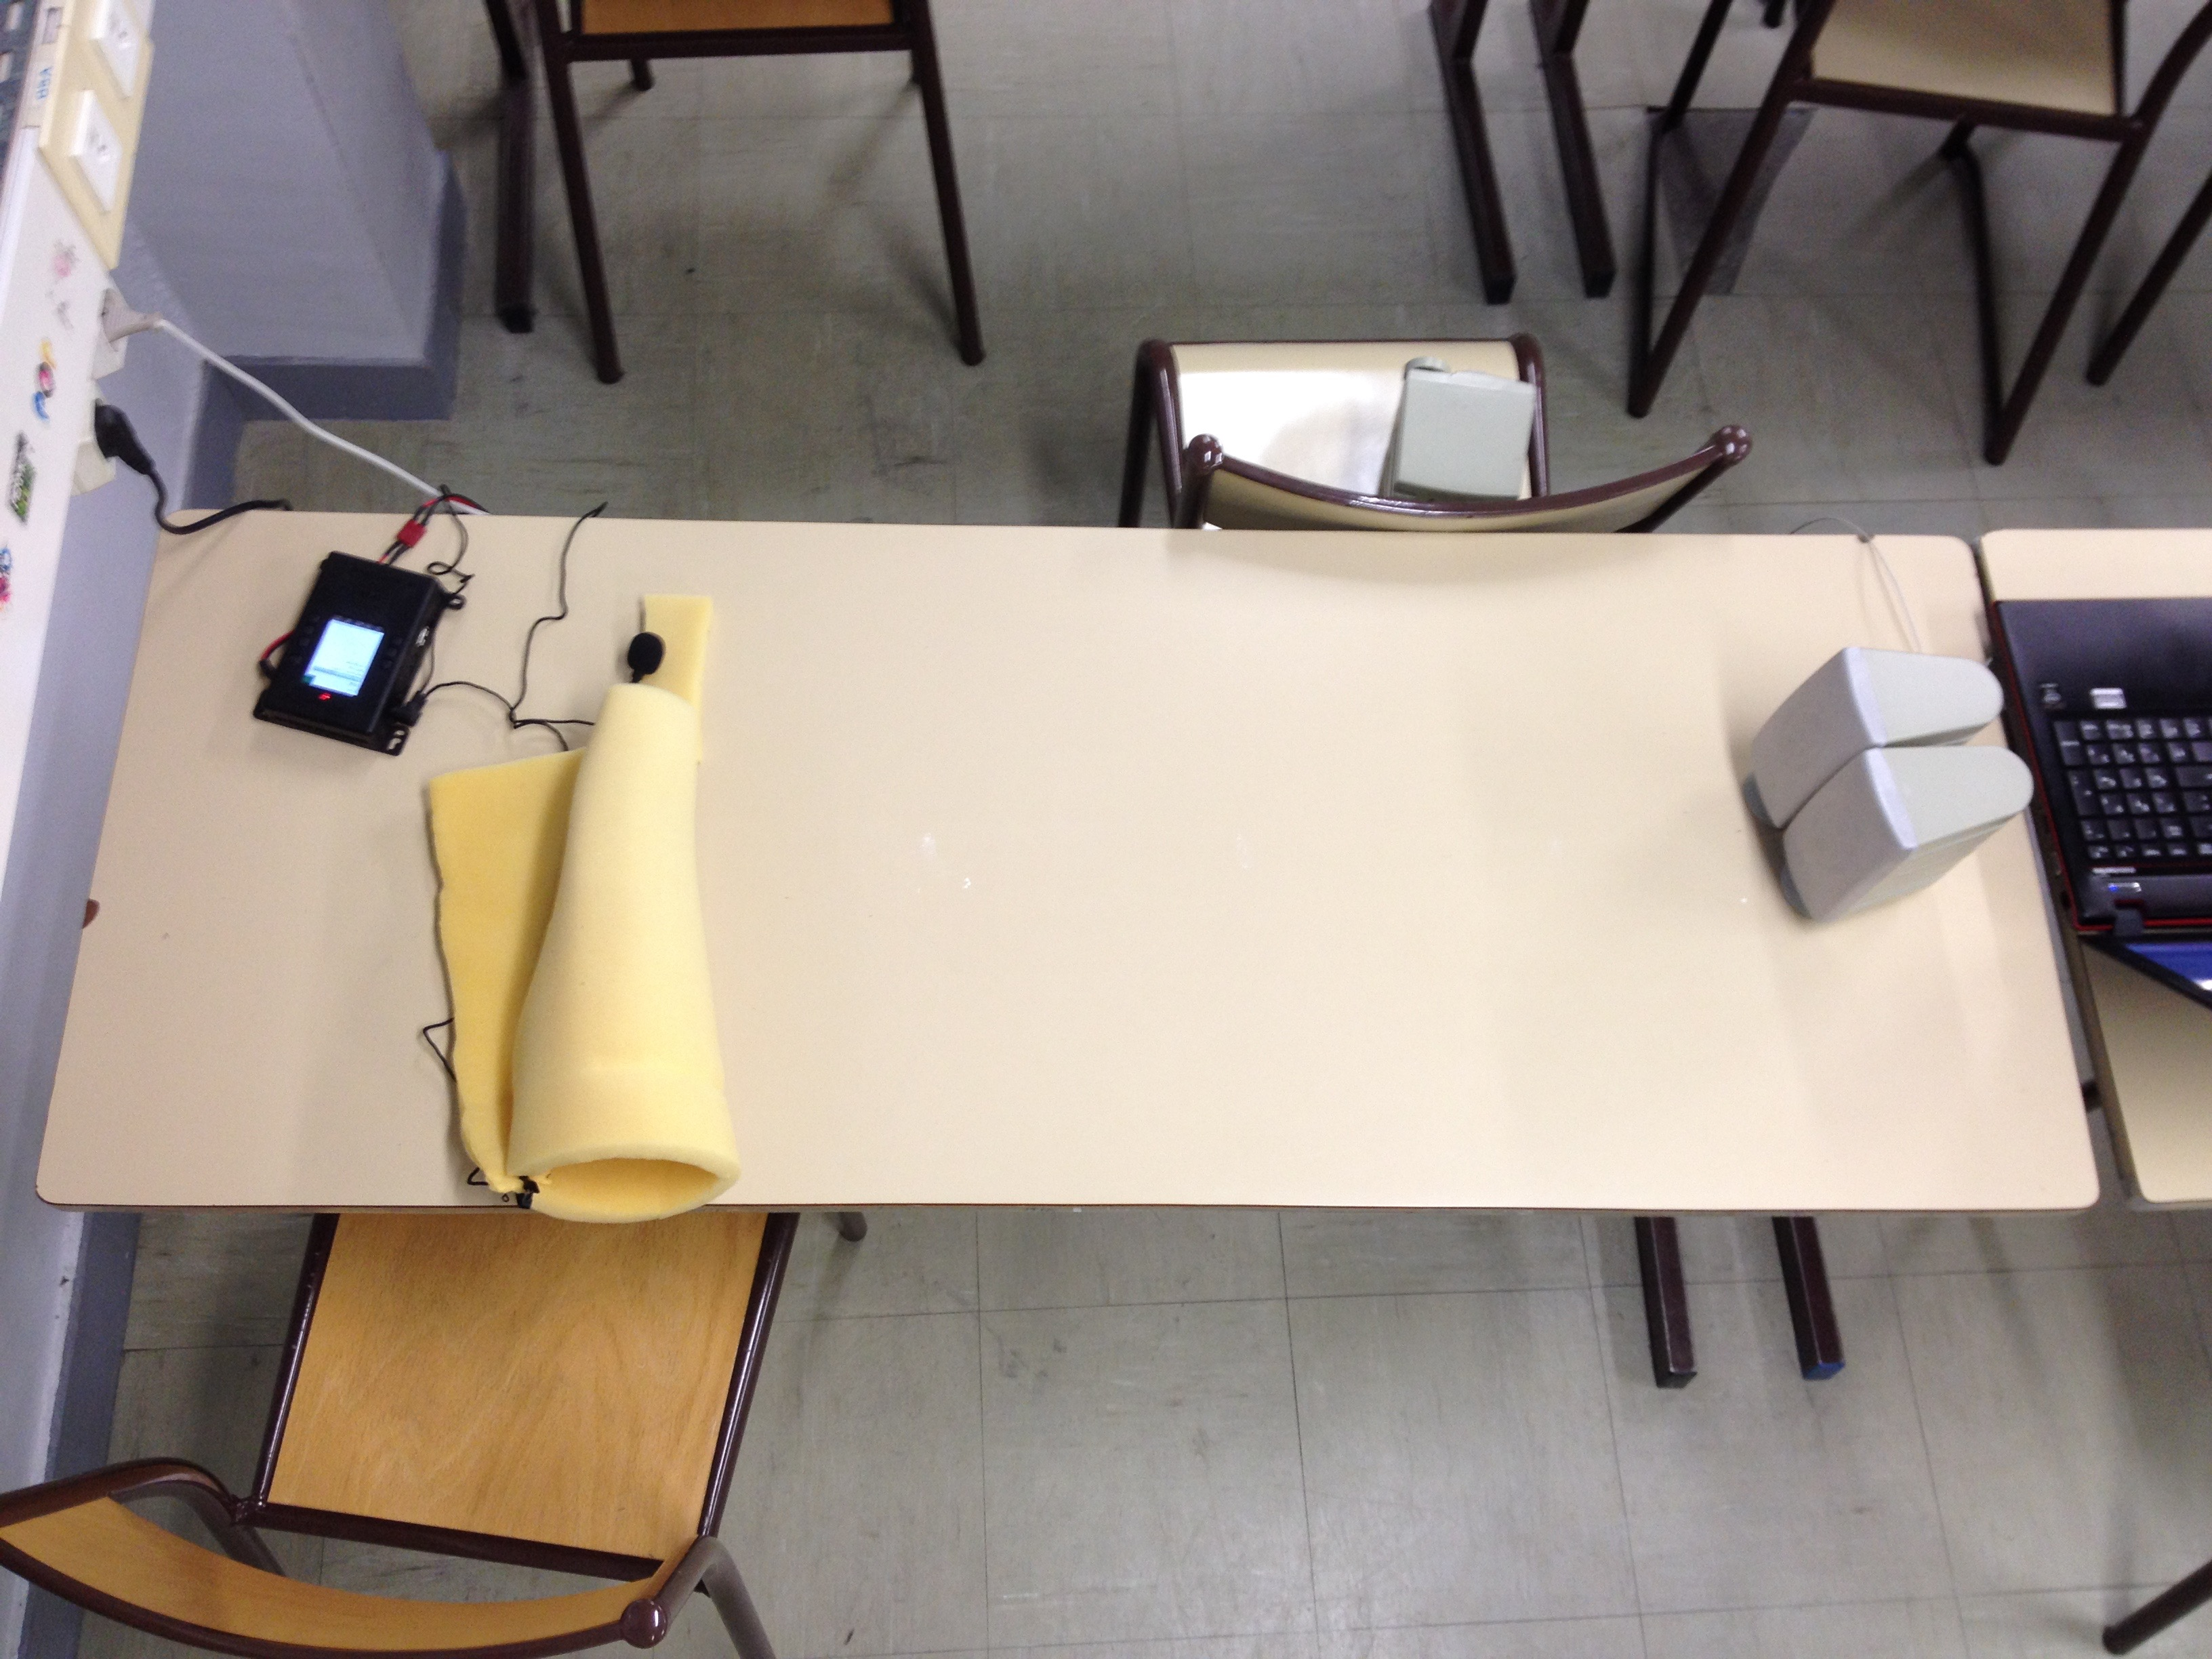
\includegraphics[width=\textwidth]{../tests/test_du_protocole/cone_dos_a_dos.jpg} 
\end{figure}


\subsubsection{perpendiculaire au haut-parleur}

On constate déjà qu'il y a un décalage assez marqué(anormal puisque les micros sont côte à côte)
\begin{figure}[h]
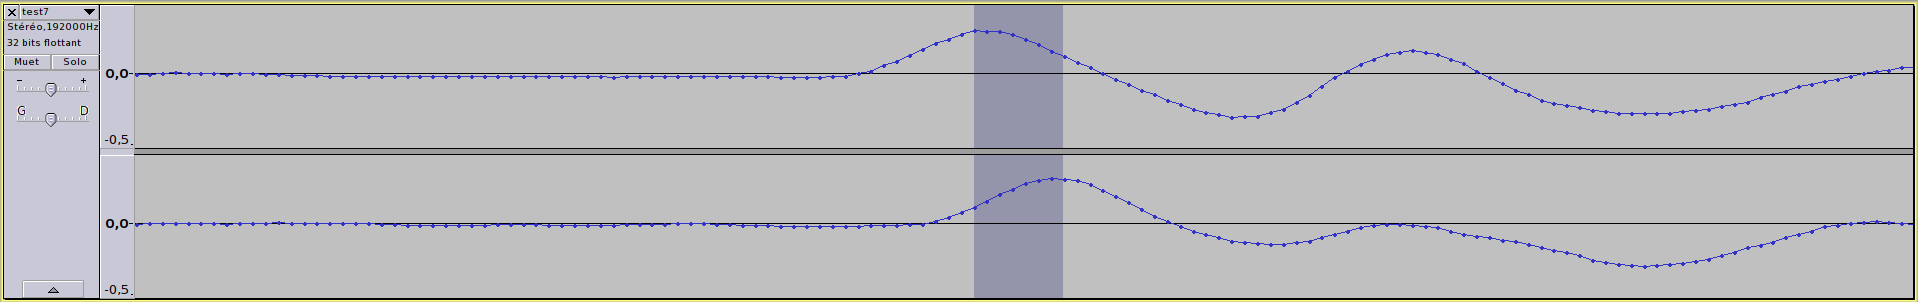
\includegraphics[width=\textwidth]{../tests/test_du_protocole/mesures_perpendiculaires/test7.png} 
\caption{exemple de décalage sur la 7ème itération de l'expérience}
\end{figure}

\begin{figure}[H]
\begin{center}
\begin{tabular}{|l || p{1.4cm} | p{1.4cm} | p{1.4cm} | p{1.7cm} | p{1.7cm}  |}
\hline
\# & $f$ (Hz) &  durée (s) & décalage de phase (échantillons) & décalage de phase (s) & décalage de phase (m)\\
\hline
\hline
1	&80	&3	&28 &0.00063	&0.2142\\
2	&80	&3	&6	&0.00014	&0.0476\\
3	&80	&3	&6	&0.00014	&0.0476\\
4	&80	&3	&6	&0.00014	&0.0476\\
5	&80	&3	&6	&0.00014	&0.0476\\
6	&80	&3	&6	&0.00014	&0.0476\\
7	&80	&3	&6	&0.00014	&0.0476\\
8	&80	&3	&6	&0.00014	&0.0476\\
9	&80	&3	&7	&0.00016	&0.0544\\
10	&80	&3	&6	&0.00014	&0.0476\\
\hline
\multicolumn{4}{|c|}{Moyenne} & 0.000191	&0.06494\\
\hline

\end{tabular}
\end{center}
~\\
où : 
\begin{description}
\item[$f$] est la fréquence utilisé.
\item[$x$] est la distance entre la source sonore et le premier micro
\item[$y$] est la distance entre les deux micros
\end{description}
\caption{tableau des résultats de toutes les itération de l'expérience avec les micros collé}
\end{figure}


\subsubsection{dos au haut-parleur}

\begin{figure}[H]
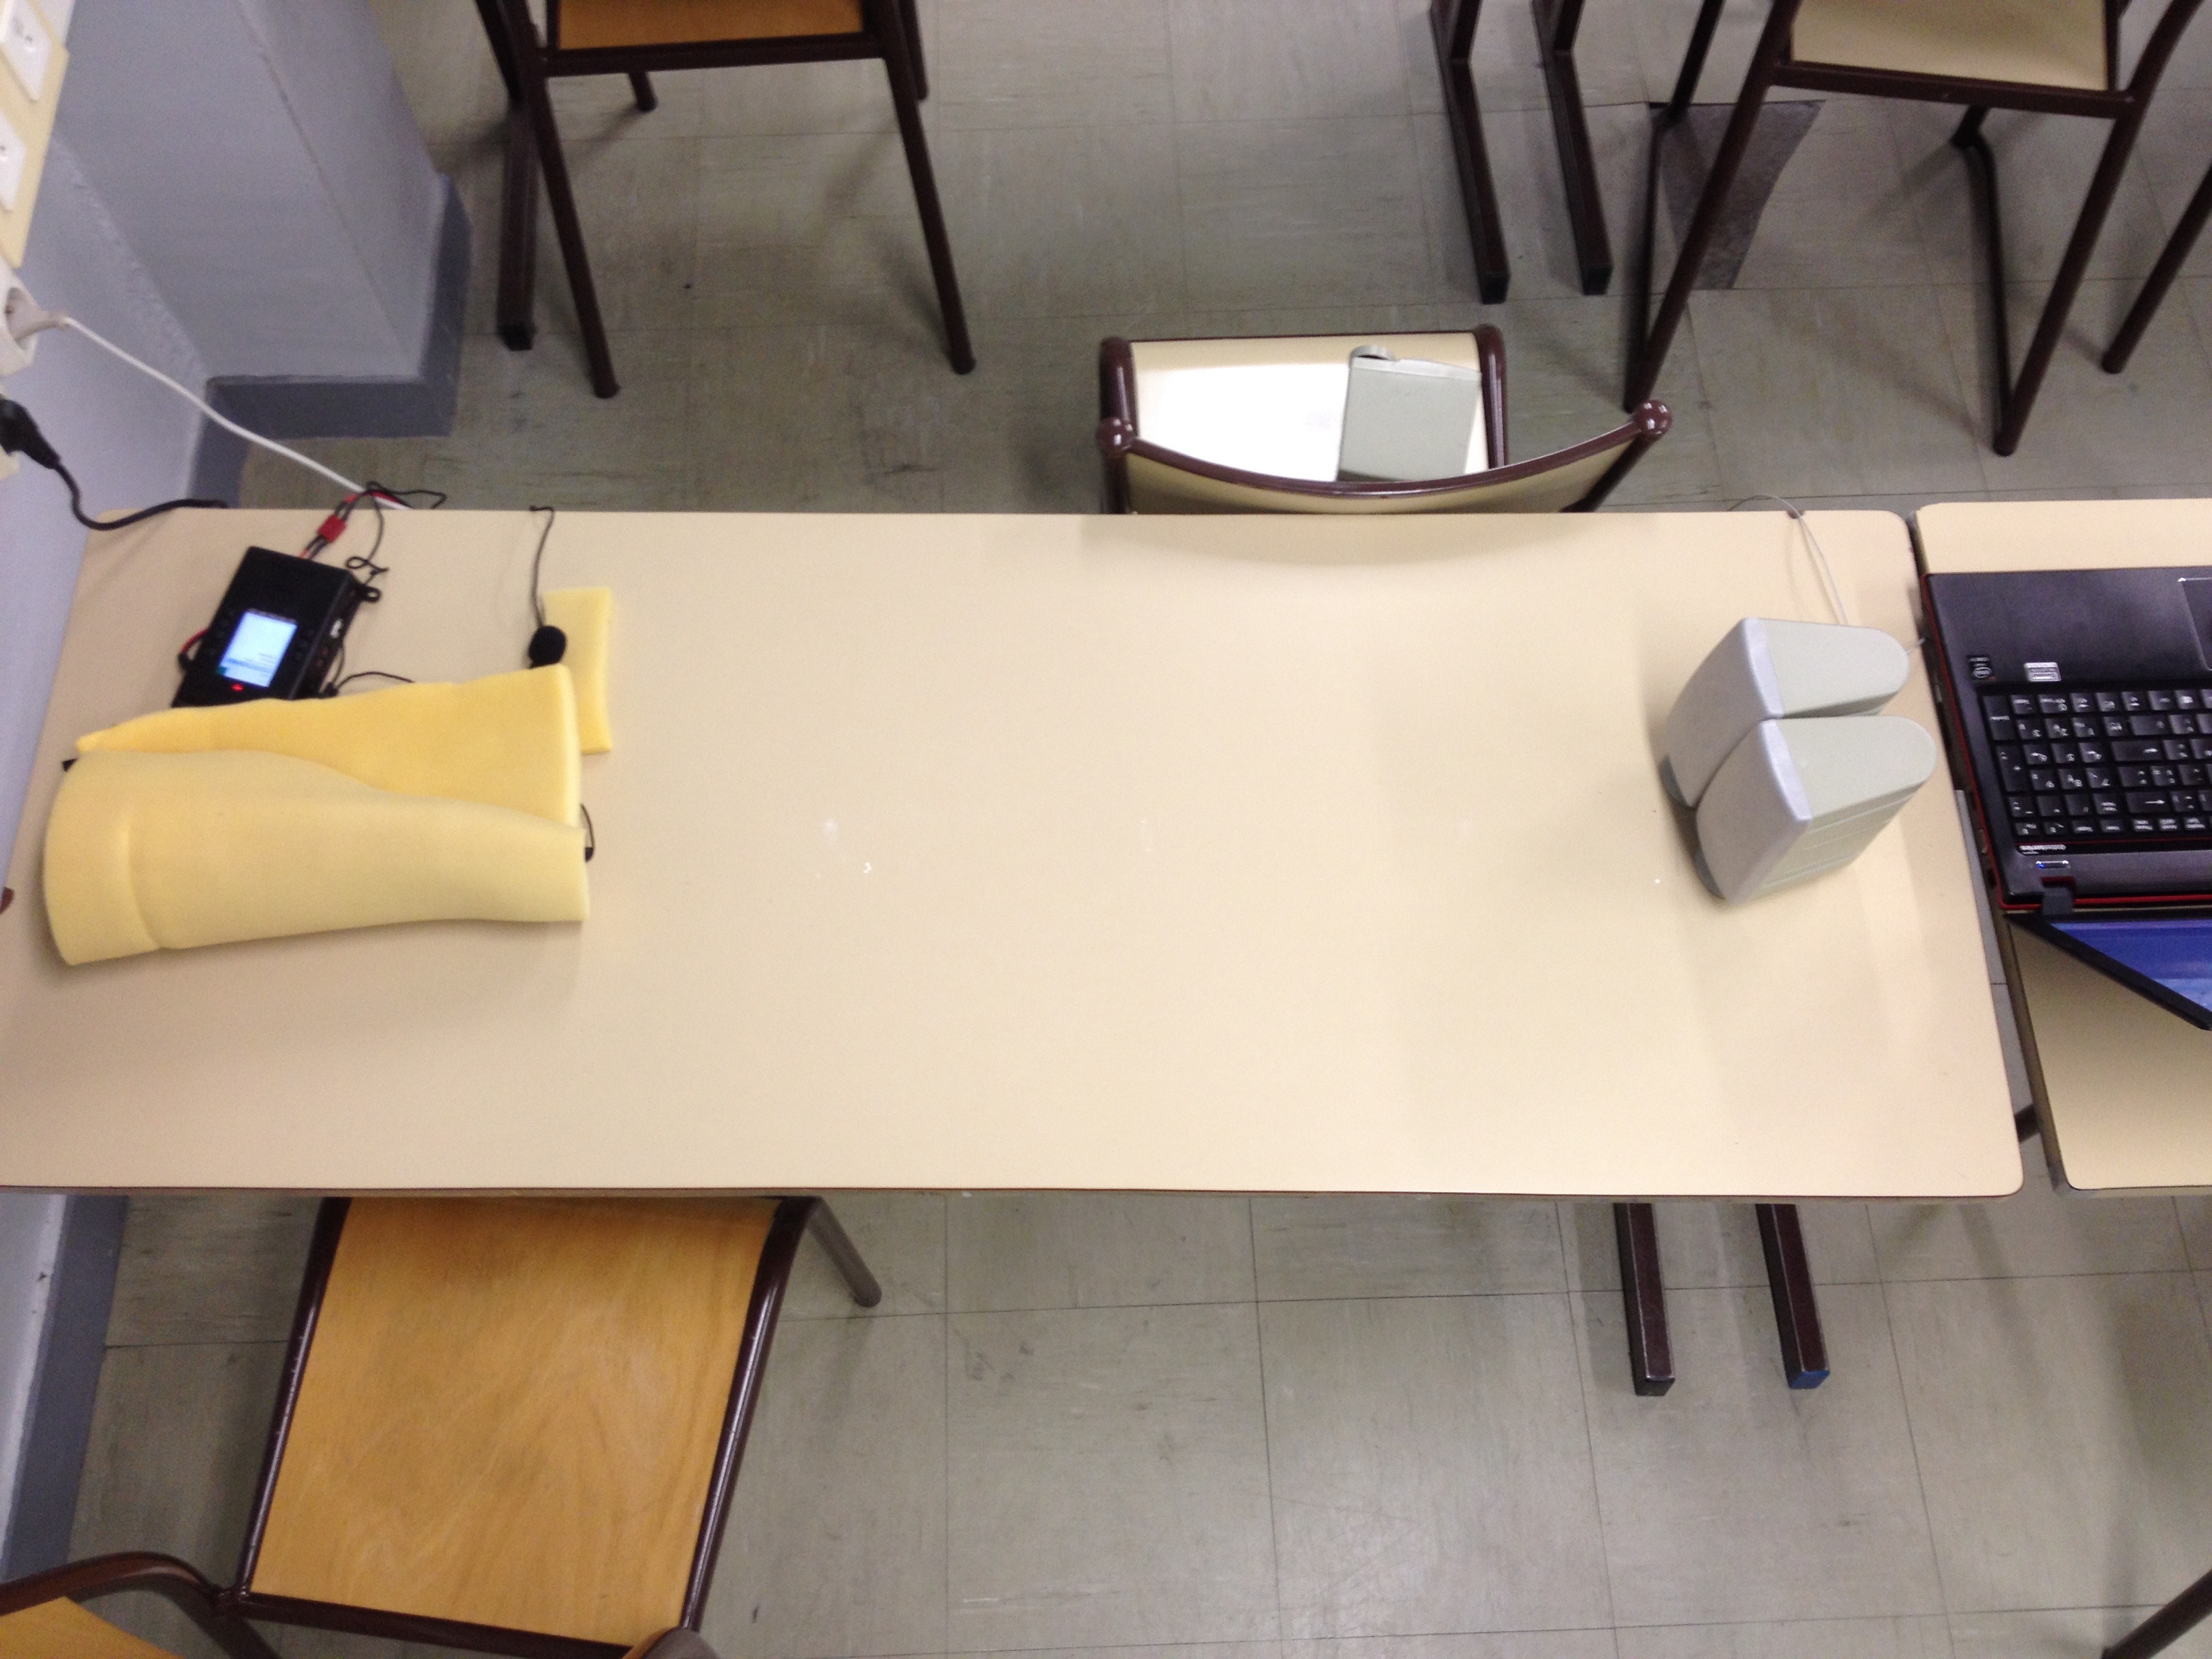
\includegraphics[width=\textwidth]{../tests/test_du_protocole/IMG_0924.jpg} 
\end{figure}

TODO: on n'a pas de données pour celui là ?

\subsection{conclusion}
On en conclu que l'écho influence effectivement beaucoup le signal reçu, pouvant fausser les calculs basés sur le décalage de phase.


\chapter{Influence de l'environnement sur l'utilisation des cônes}
\section{Objectif}
Au cours d'une expérience précédente on s'est rendu compte que dans certains cas, même en utilisant des cônes, le signal reçu était fortement bruité (très probablement par accumulation d'écho). On aimerait savoir si ce problème provient de l'environnement (en l'occurrence une grande pièce sans obstacles) et si on peut améliorer le signal en modifiant le cône.

\section{Expérience}
\subsection{Critères d'acceptation}
On partira de la capture du signal quasi inexploitable et on comparera les nouveaux résultats avec celui-ci et le signal émis pour voir s'il y a une amélioration ou pas.
\begin{figure}[H]
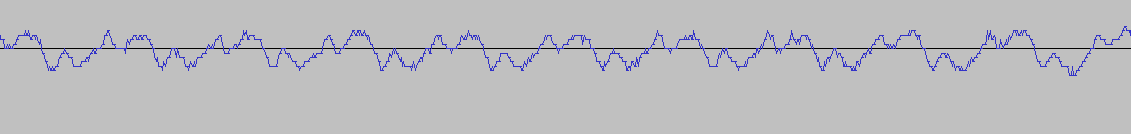
\includegraphics[width=\textwidth]{resources/img/cone_90.png}
\caption{le signal bruité}
\end{figure}
\begin{figure}[H]
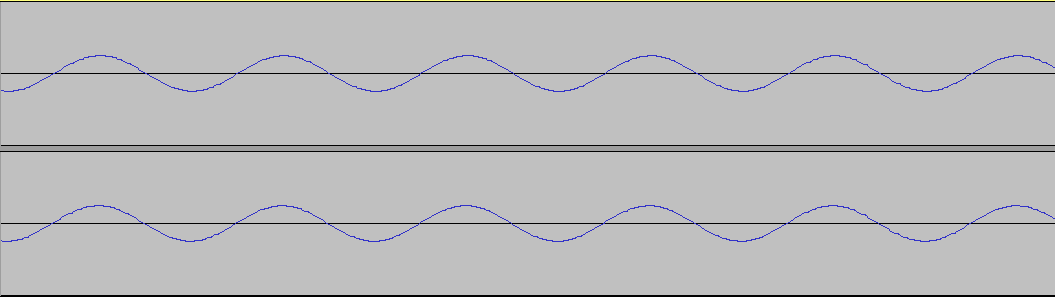
\includegraphics[width=\textwidth]{resources/img/sinus_base.png}
\caption{le signal de base}
\end{figure}
On regardera le milieux/la fin du signal reçu, afin d'être sûr que l'écho ait bien eu le temps de s'ajouter au signal de base.


\subsection{Configurations physique}
On utilise un seul micro, perpendiculaire à l'émetteur et dans un cône de mousse.

On testera avec un cône le moins ouvert possible (cylindre) pour voir si on peut réduire l'écho perçu.

Puis on mettra un obstacle à 80 centimètres de la sortie du cône pour simuler un environnement plus étroit.

\subsection{environnement de test}
Les tests se font dans une grande pièce sans obstacles(pas à la hauteur où se passe l'expérience du moins).

\subsection{Signal émis}
même sinusoïde que pour \ref{protocole}, seulement elle dure 10 secondes.

\subsection{Réception du signal}
même chose que dans \ref{protocole}.

\section{Résultats}
\subsection{Cône plus refermé}
\begin{figure}[H]
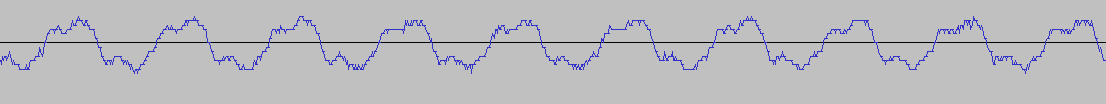
\includegraphics[width=\textwidth]{resources/img/cone_90_plus_fin.png}
\caption{utilisation d'un cône plus refermé}
\end{figure}
Le fait d'utiliser cône plus refermé semble améliorer le signal reçu, il reste quand même très bruité.

\subsection{Ajout d'un obstacle}
\begin{figure}[H]
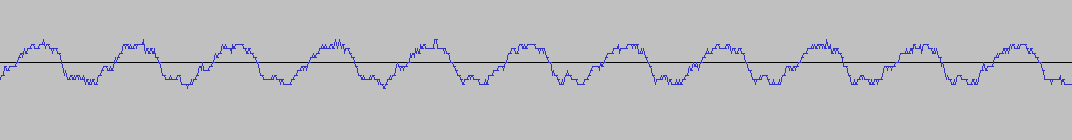
\includegraphics[width=\textwidth]{resources/img/cone+obstacle.png}
\caption{signal avec un obstacle en face de la sortie du cylindre}
\end{figure}
Cette fois la forme du signal ressemble beaucoup plus au sinus de base.

\section{Conclusions}
Utiliser un cylindre plutôt qu'un cône semble améliorer un peu le signal.

L'environnement semble jouer un grand rôle dans le signal perçu, dans un environnement ouvert comme c'était le cas au début, on a beaucoup d'écho, alors qu'en rajoutant simplement un obstacle à 80cm de la sortie du cylindre  on obtient un signal bien plus exploitable, il faudrait creuser plus en regardant si ça marche pour tout types d'obstacles (forme/matériau) et jusque quelle distance.


\chapter{Signal carré}\label{signal_carre}
\section{Objectifs}
Le premier objectif de cette série de tests est de vérifier la validité de l'utilisation d'un signal carré.
On a voulu tester cette forme de signal, car le front montant du signal est supposé être facilement repérable dans le signal de l'acquisition du micro. \\
Le deuxième objectif est d'acquérir un signal avec le minimum d'écho possible. Le signal carré utilisé étant très court, le pique enregistré sur les micros ne devrait (hypothétiquement) pas être bruité par de l'écho.

\section{Protocole}\label{protocole}
On a créé deux fichiers $.wav$:
\begin{itemize}
\item Le premier envois 4 impulsions  de longueur 1 échantillon, espacé de 3 secondes chacun
\item Le deuxième envois 4 impulsions de longueur 5 échantillons, espacé de 3 secondes chacun
\end{itemize}
On a ensuite fait les mêmes teste que pour les séances précédentes:

\subsection{Protocole des tests}
 
 \paragraph{Premier test} 
 Les deux micros sont côte à côte(à 6cm de décalage), à la même distance de la source sonore.
 \subparagraph{Objectif du test}
 Ce test est réalisé pour avoir une référence par rapport aux autres test. En plus d'une référence, ce test permet de voir les différence d'acquisition là où il ne devrait pas en avoir.
 \begin{figure}[H]
 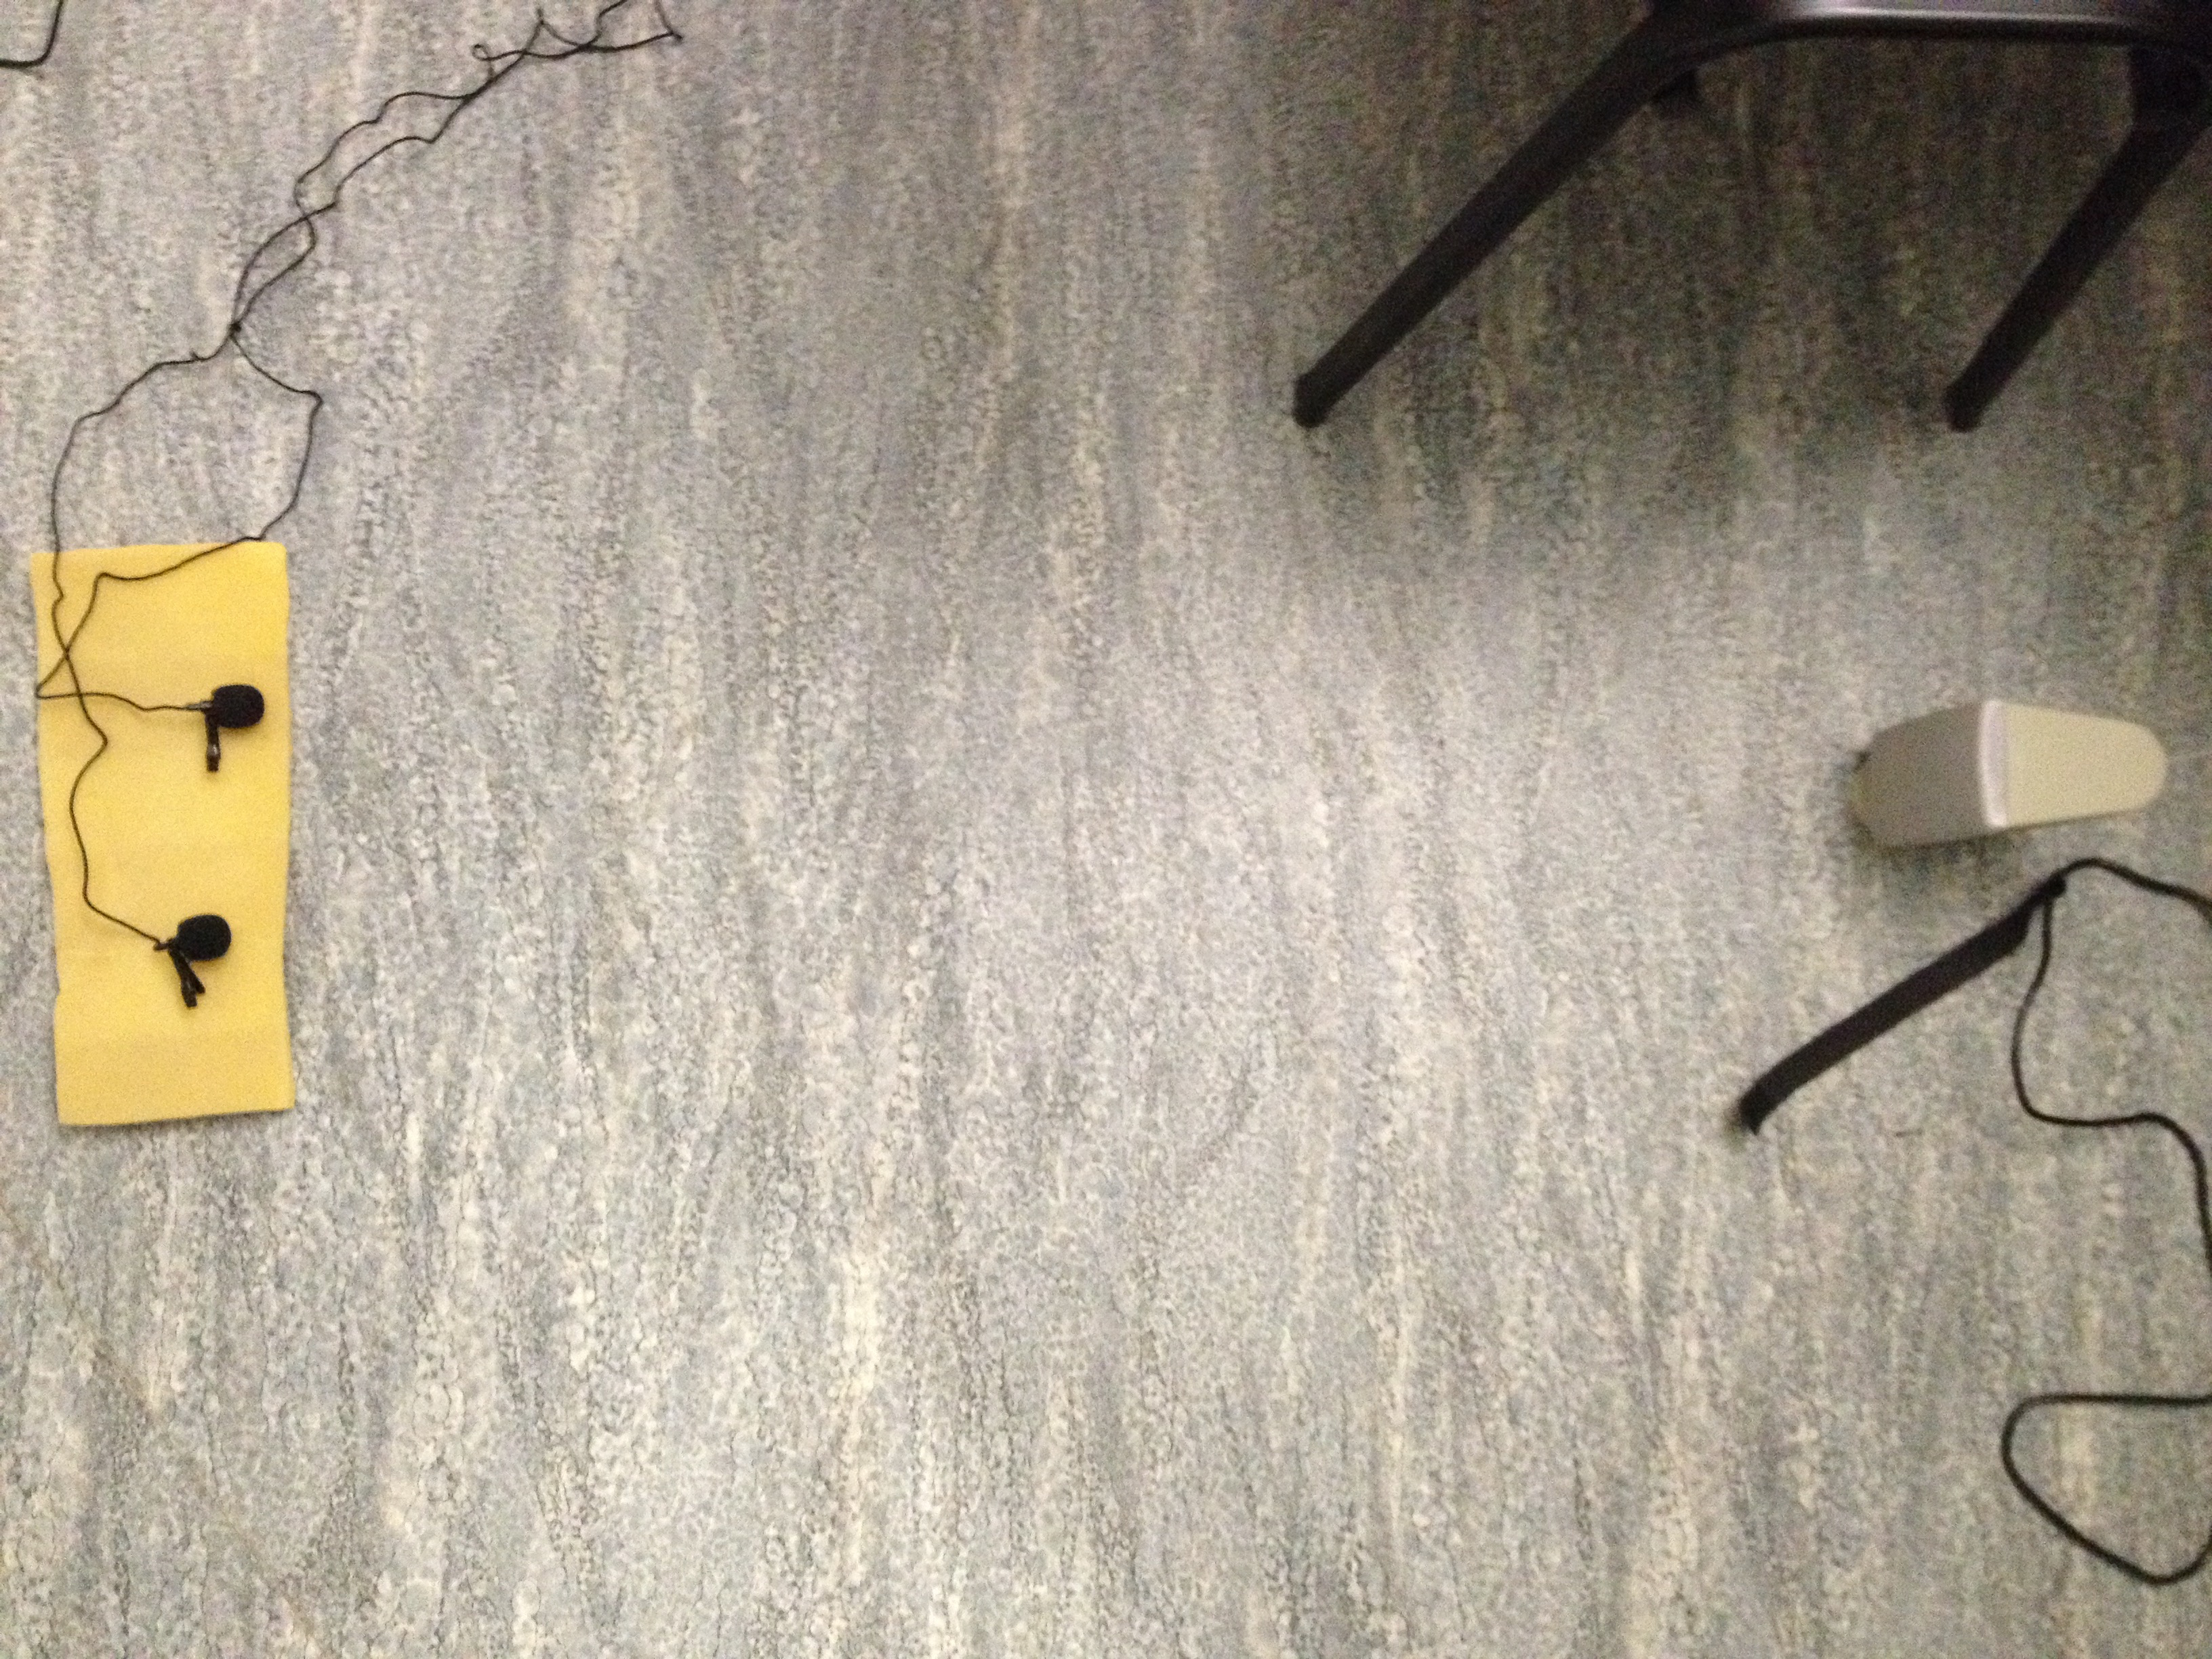
\includegraphics[width=\textwidth]{../tests/lecture_de_signaux_carres/donnees11-03/test_1.jpg} 
 \caption{Photo de l'expérience avec les micros côte à côte}
 \end{figure}
 	
 \paragraph{Deuxième test} 
 Les deux micros sont en ligne droite avec le haut-parleur. La distance entre les deux micros est de 520mm, la distance entre le micro le plus proche du haut-parleur et le haut-parleur est de 400mm.
 \subparagraph{Objectif du test}
 Le but de ce test est de vérifier qu'on arrive à obtenir le bon resultat sur le calcul de distance entre les deux micros à partir du décalage de phase.
 \begin{figure}[H]
 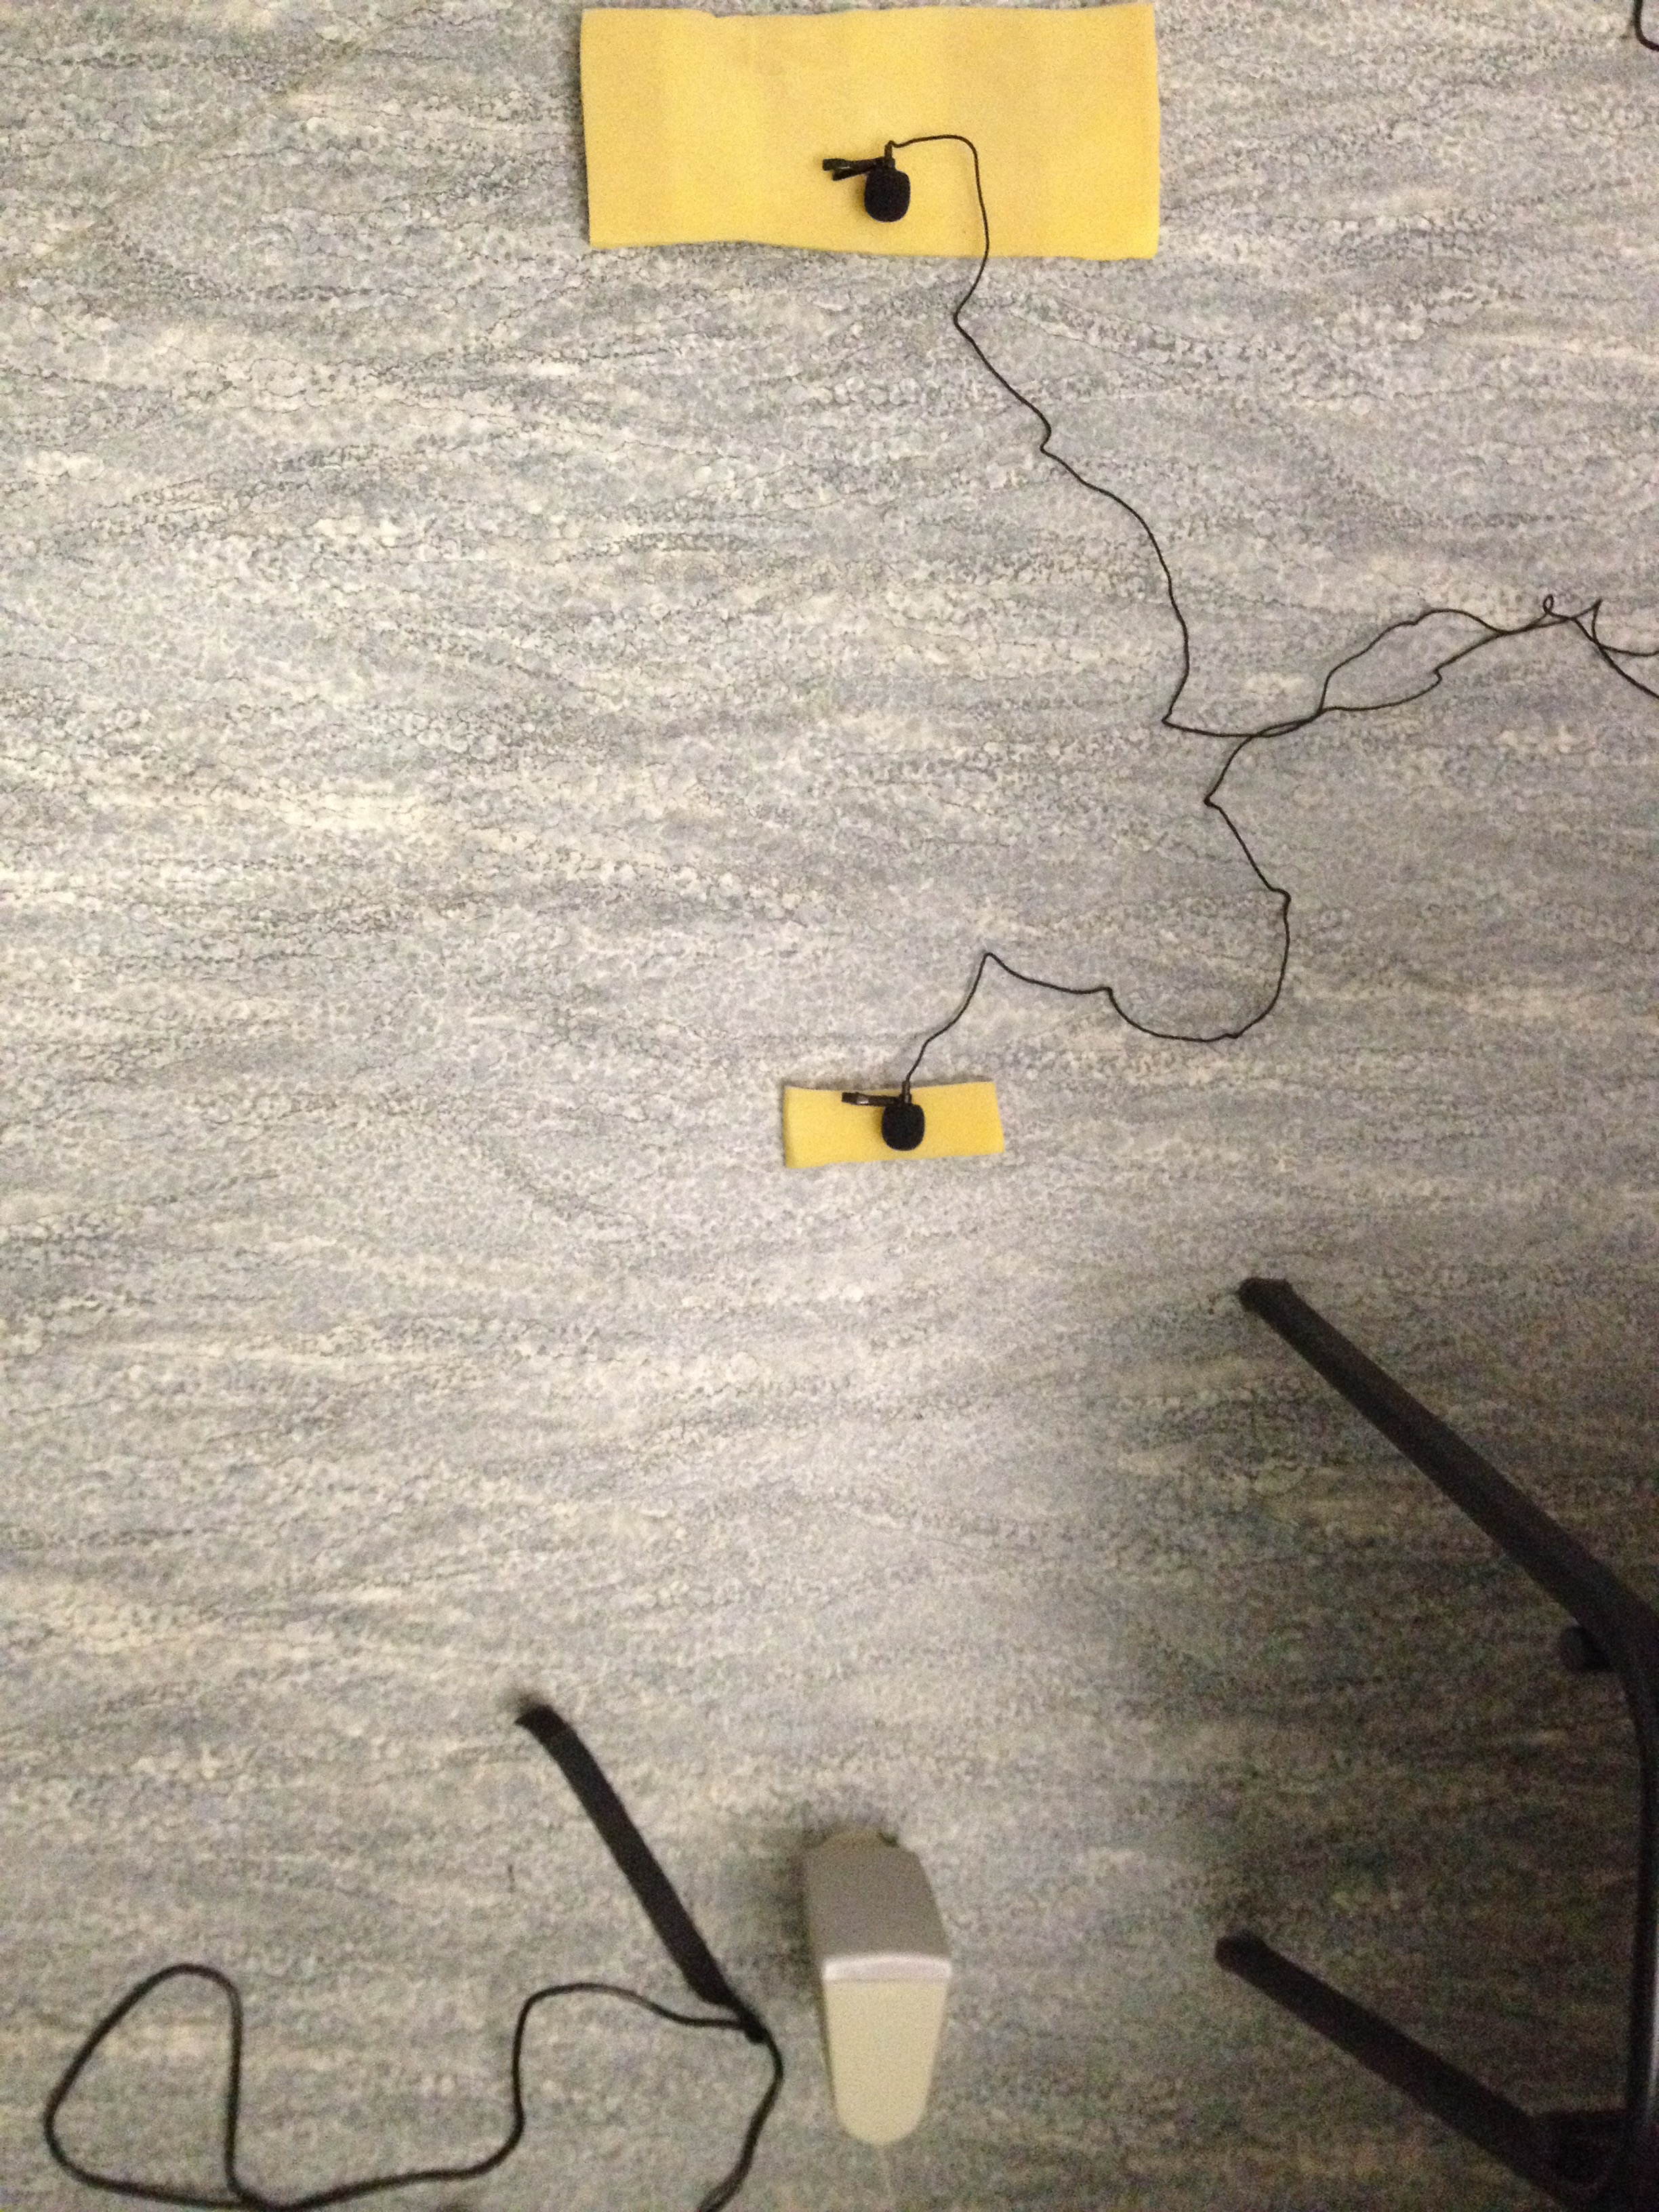
\includegraphics[width=\textwidth]{../tests/lecture_de_signaux_carres/donnees11-03/test_2.jpg} 
 \caption{Photo de l'expérience avec les micros en ligne}
 \end{figure}
 	
 \paragraph{Troisième test} 
 Les deux micros sont à la même distance par rapport à la source sonore (920mm), mais il sont tous deux séparé de 680mm.
 \subparagraph{Objectif du test}
 Le but de ce test est de voir comment se propage le son en direction des deux micros. En effet, le haut-parleur n'est pas complètement omnidirectionnel, on voudrait savoir si cela a un effet important sur le signal. En plus d'impacter le signal perçu directement, cela peut aussi changer l'écho perçu par les micros. 
 \begin{figure}[H]
 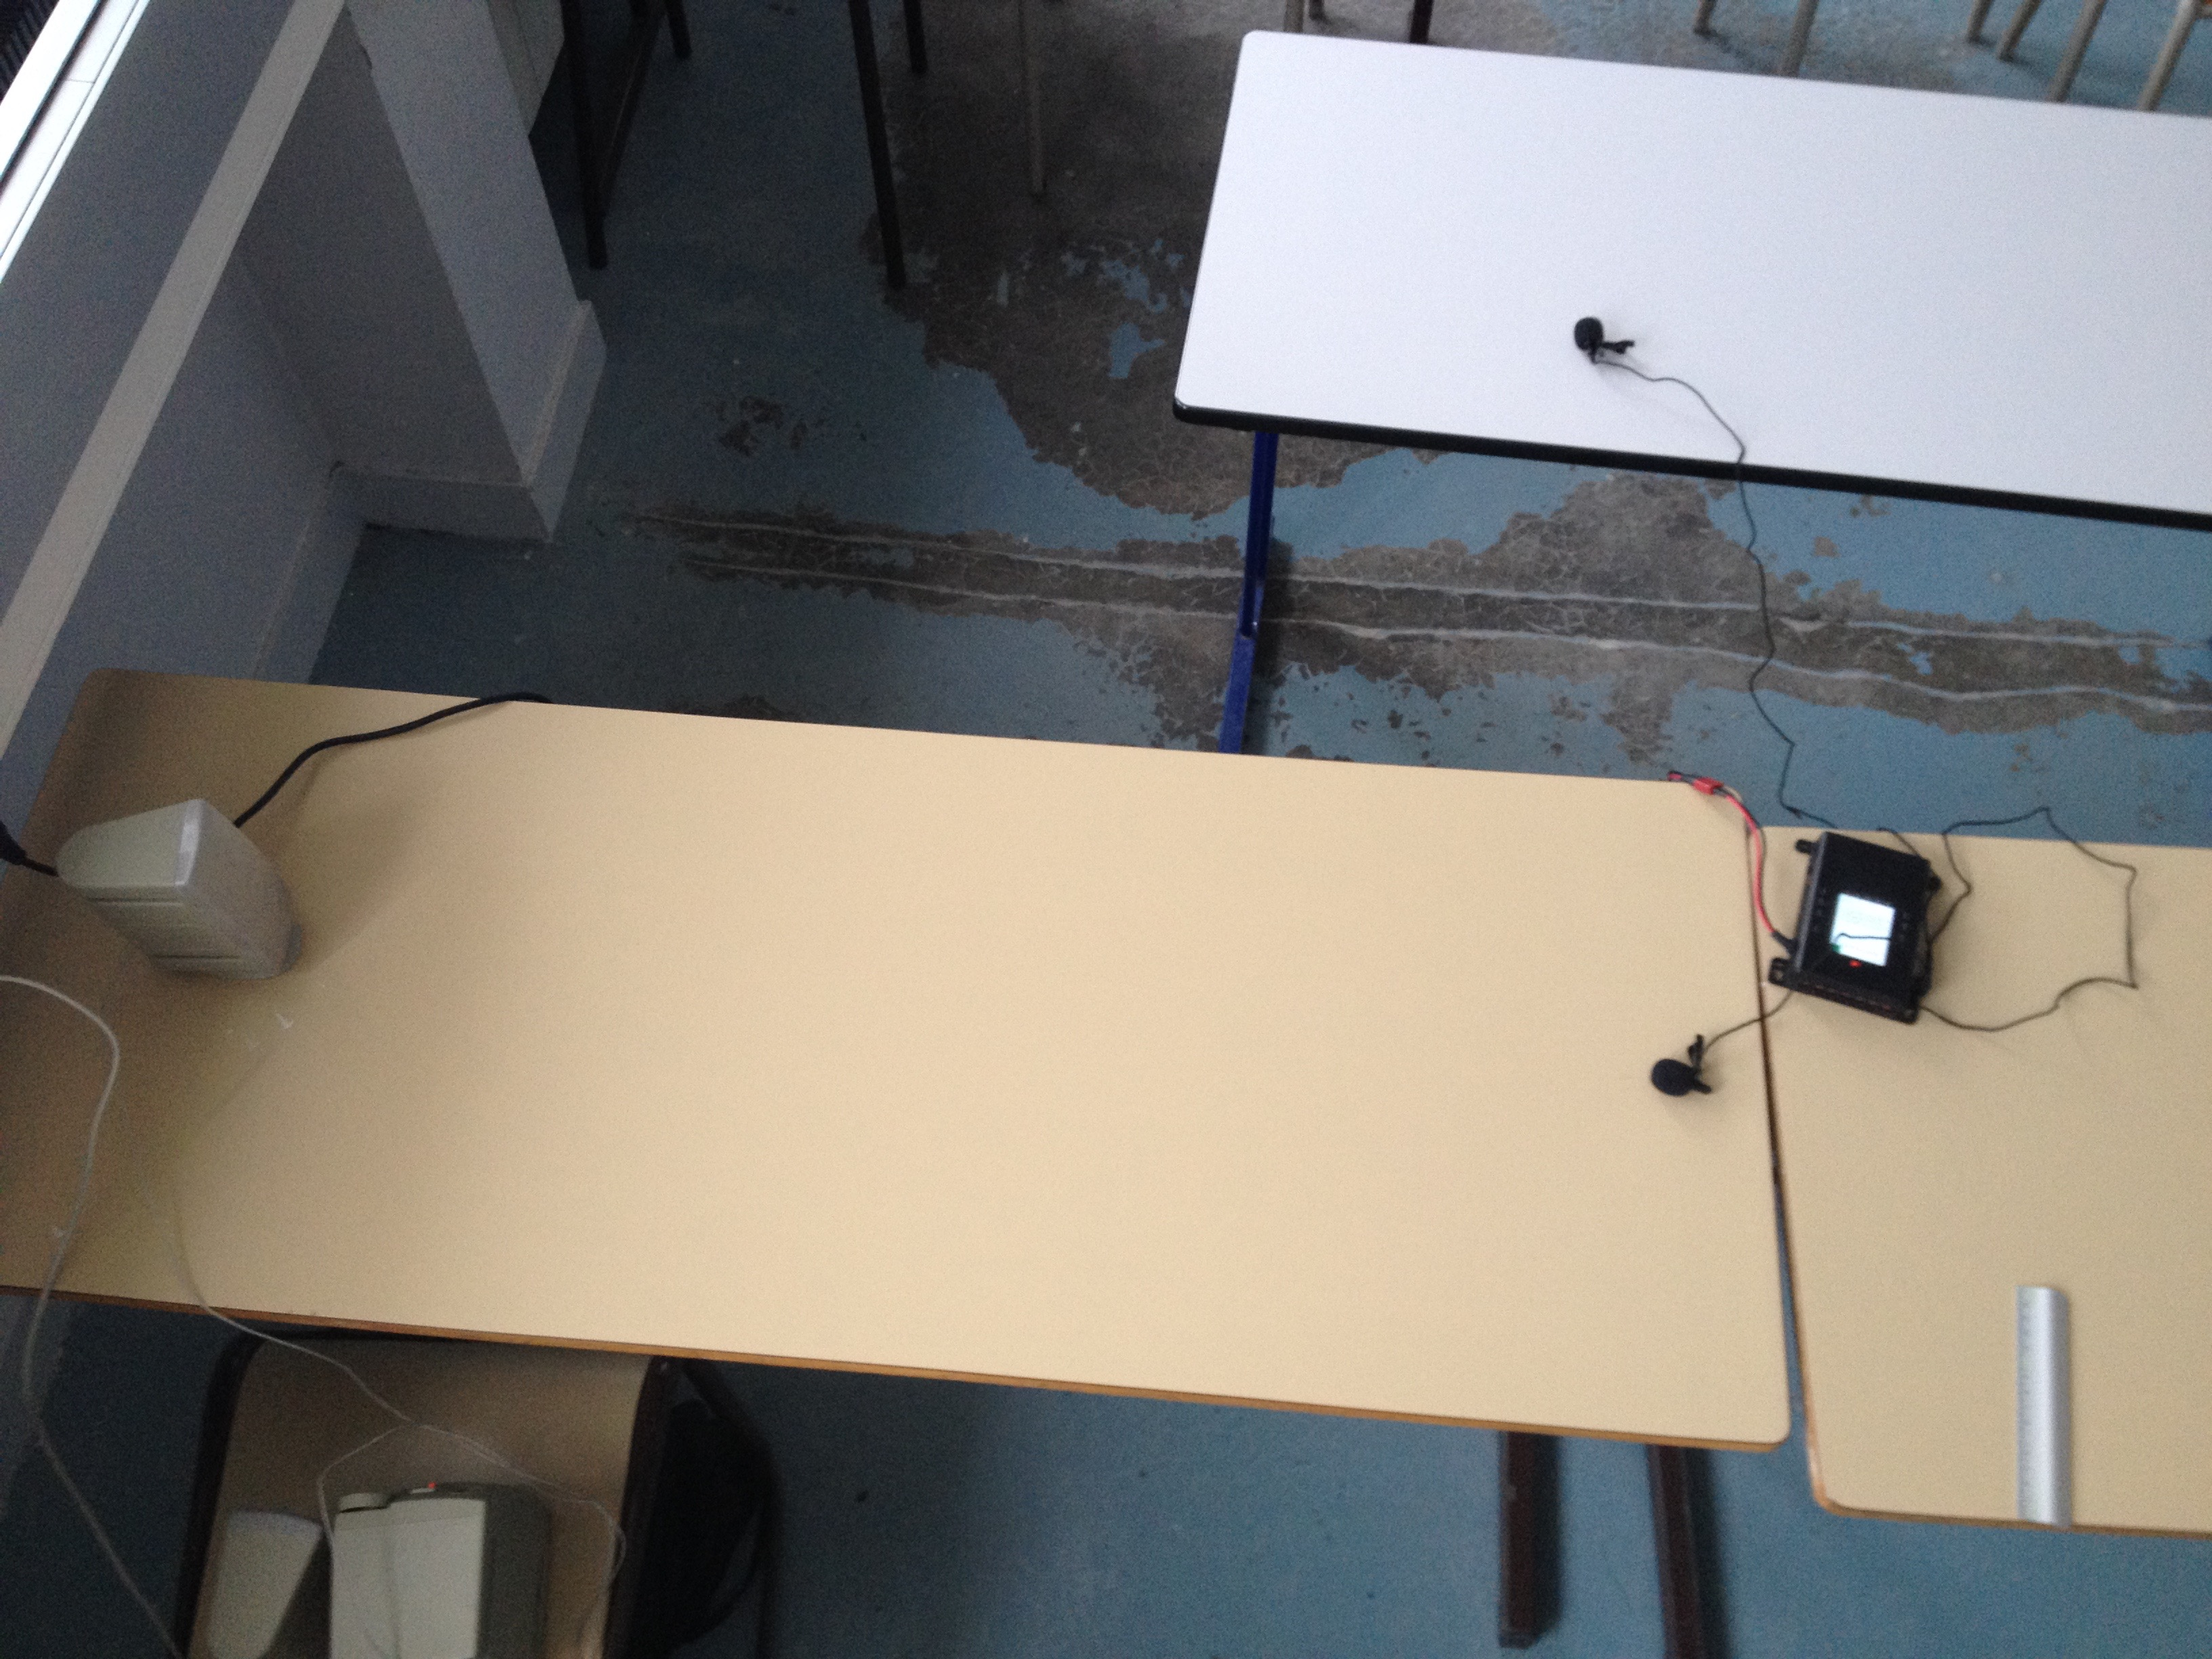
\includegraphics[width=\textwidth]{../tests/lecture_de_signaux_carres/donnees11-03/test_3.jpg} 
 \caption{Photo de l'expérience avec les micros à la même distance de la source, mais séparés}
 \end{figure}
 
 \paragraph{Quatrième test} 
 Un des deux micros est entouré de mousse pour faire un cône, le rendant unidirectionnel. Le cône est dirigé vers le haut-parleur. Les deux micros sont à une distance de 900mm de la source sonore. Les deux micros sont séparé de 12cm.
 \subparagraph{Objectif du test}
 Le but de ce test est de comparer ce que les deux micros acquire. En effet, l'un des deux micro devrait etre moins impacter pas l'écho ambiant, et donc etre moins bruité.
 \begin{figure}[H]
 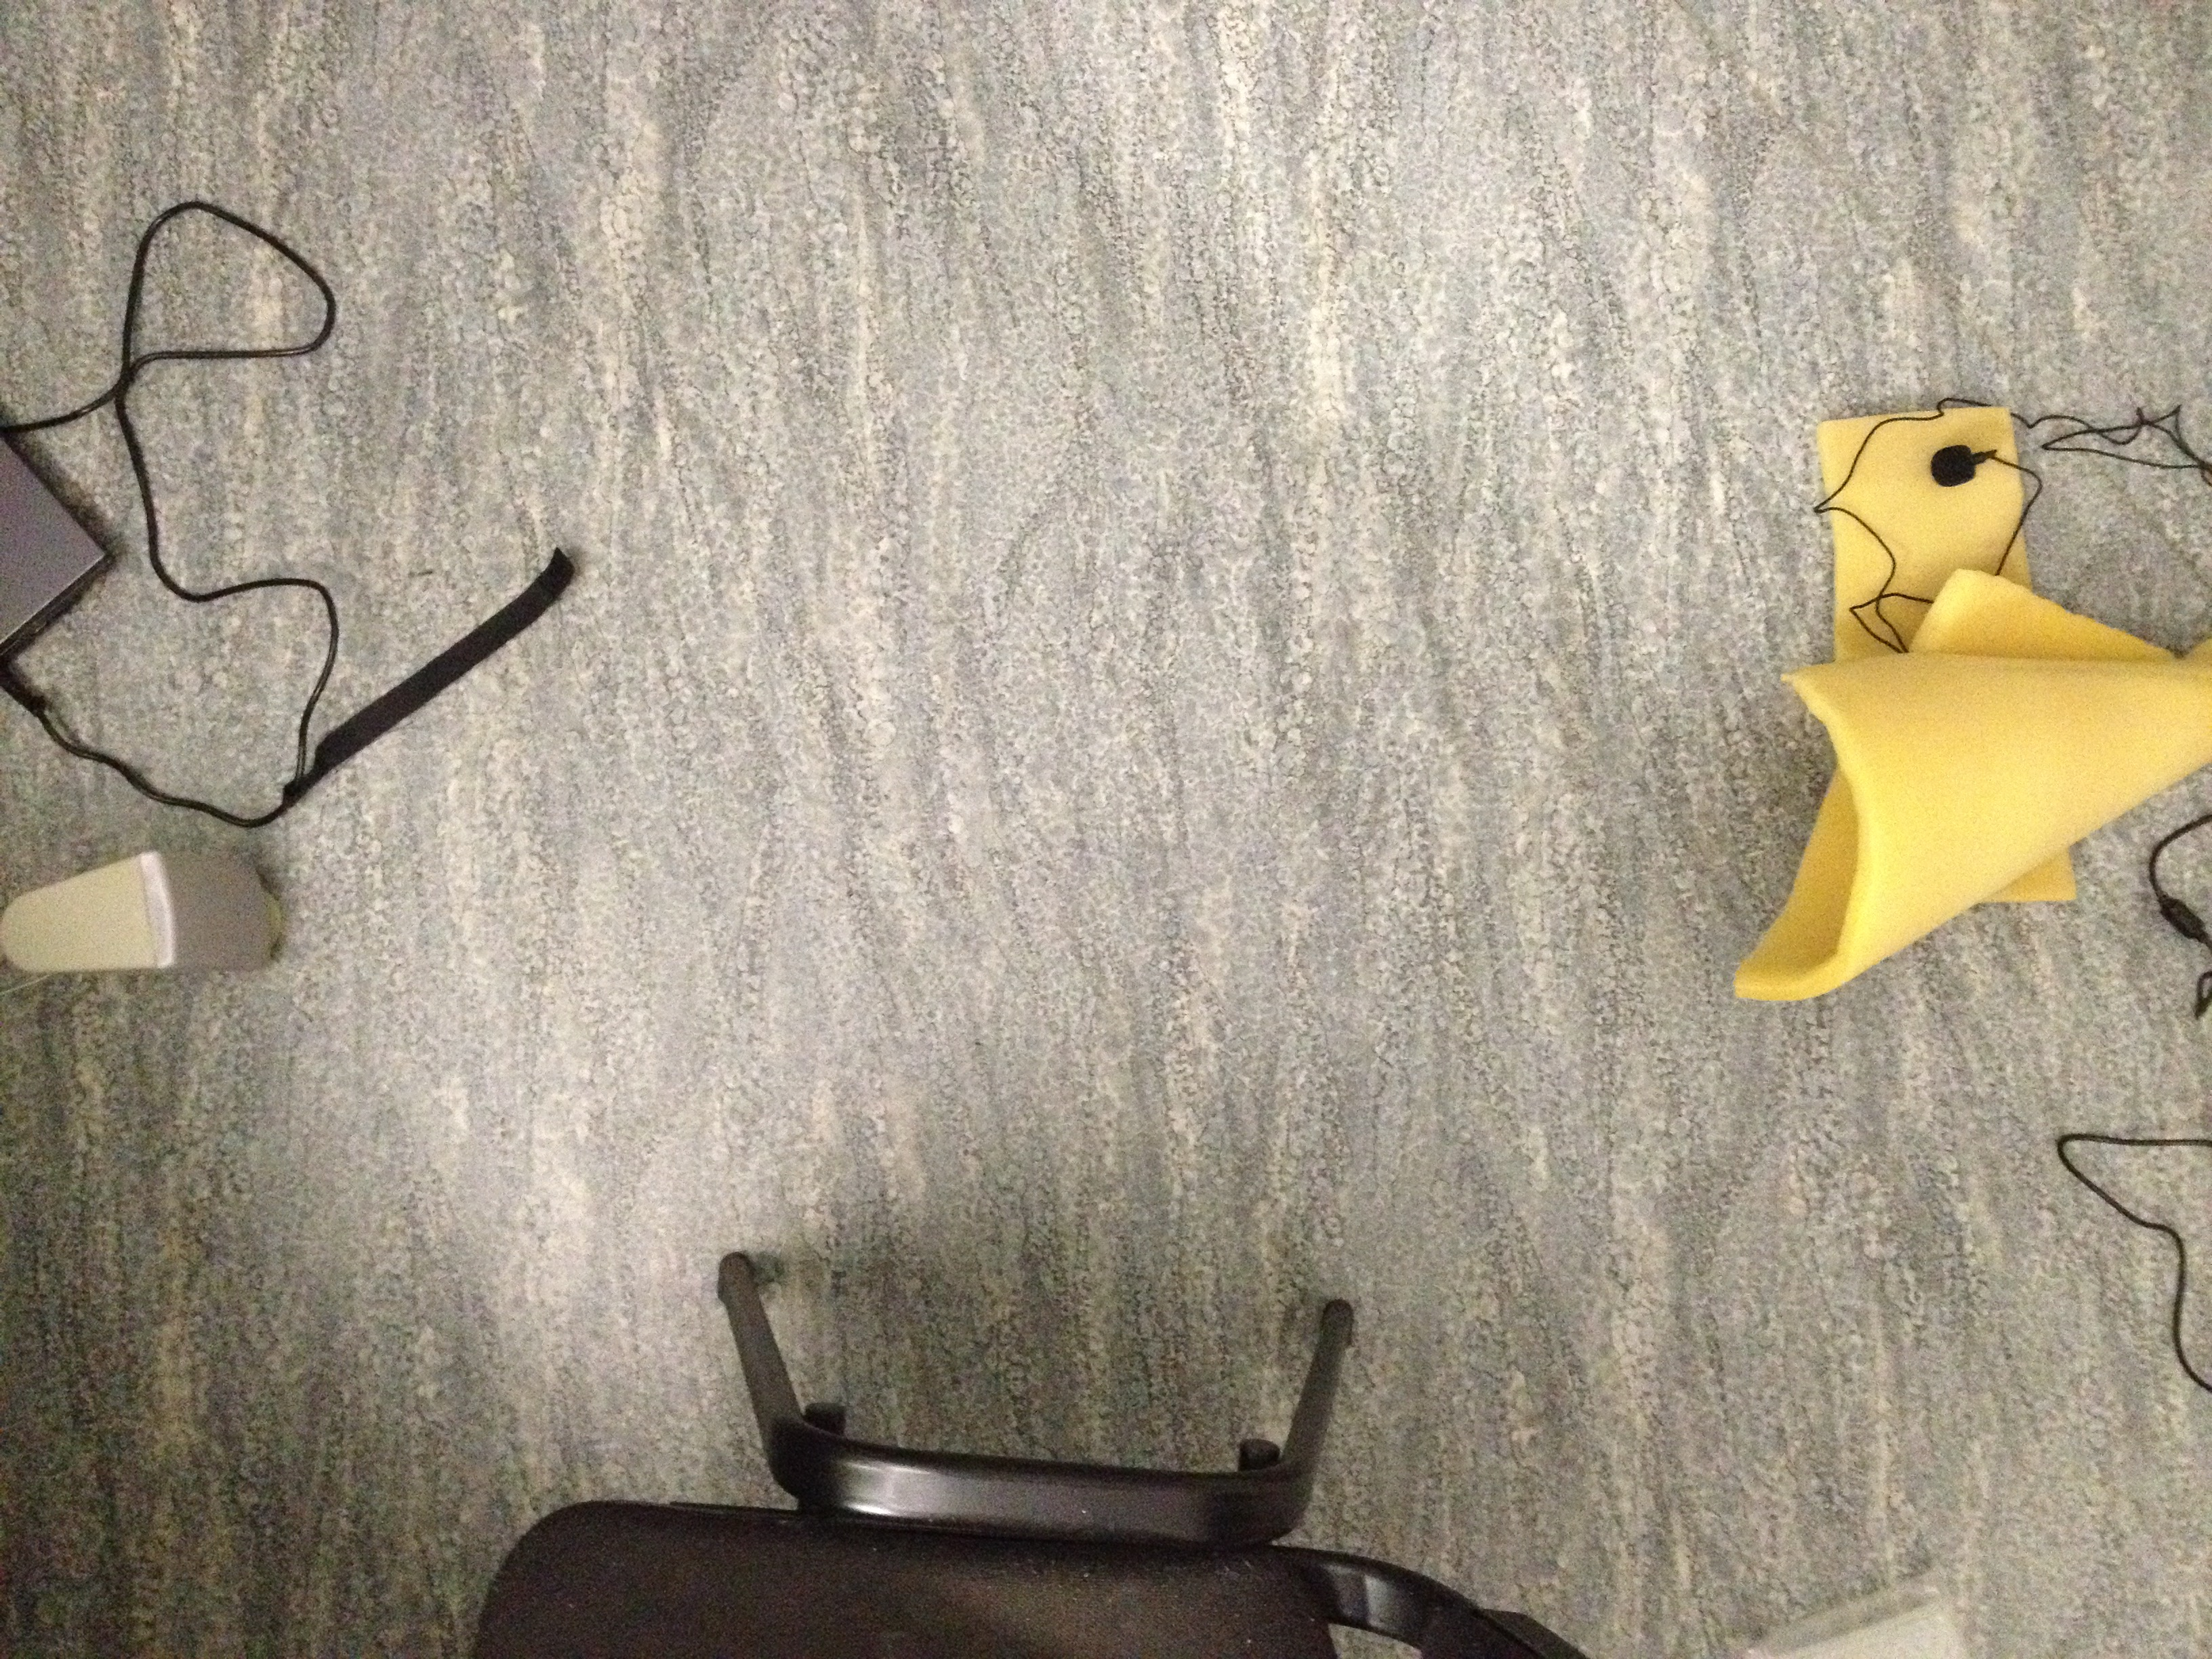
\includegraphics[width=\textwidth]{../tests/lecture_de_signaux_carres/donnees11-03/test_4.jpg} 
 \caption{Photo de l'expérience avec un cône autour d'un micro}
 \end{figure}
 	
 \paragraph{Cinquième test} 
 Un des deux micros est entouré de mousse pour faire un cone, le rendant unidirectionnel. Le cône est dirigé à 180 degré du haut-parleur. Les deux micros sont à une distance de 900mm de la source sonore.
 \subparagraph{Objectif du test}
 Le but de ce test est de comparer les mesures entre les deux micros. L'un des micro ne pourra pas acquerir le son direct émis du haut parleur, l'enregistrement sur ce micro devrait donc etre principalement composé d'écho de la source sonore.
 


\section{Résultats/conclusions}
\subsection{résultats}
\paragraph{Impulsion carré de 1 échantillon}
\begin{description}
\item[Premier test] Il n'y a pas de décalage de phase entre les deux micros. De plus l'écho est n'apparait qu'après la fin du signal initial. Celui-ci est assez loin pour que le signal original ne soit pas bruité par l'écho
\item[Deuxième test] \label{test1sample1} Le décalage de phase est de 62 échantillons. Les signaux se ressemblent, même à partir du moment où l'écho s'est mis en place. Le signal du micro le plus éloigné est très atténue par la distance entre la source et ce micro.
\item[Troisième test] Il y a un léger décalage de phase qui pourrait être dû au haut parleur qui n'est pas omnidirectionnel. En ce qui concerne l'écho, il apparait aussi bien après le signal initial et ne le bruite pas.
\item[Quatrième test] Il y a un décalage de phase que nous n'arrivons pas à expliquer.
\item[Cinquième test] Le signale du micro avec la cone est très atténue. Meme avec le cone, le micro enregistre quand meme une partie du signal initial (même s'il est très atténue par rapport à l'autre micro). Il y a aussi un décalage de phase de 13 échantillons, ce qui est consistant avec l'orientation du micro (cf. \hyperref[orientation_micro]{Orientation des micros}). Cependant le décalage de phase entre l'acquisition du front initial par le micro sans cone, et l'écho acquerit par le micro avec un cone est de 65 échantillons (ce qui est consistant avec l'environnement de la pièce).
\end{description}

\paragraph{Impulsion carré de 5 échantillons}
\begin{description}
\item[Premier test] Il n'y a pas de décalage de phase entre les deux micros. En ce qui concerne l'écho, il n'est pas discernable, en effet le haut-parleur à du vibrer plus que ce qui était prévu. Le problème est du à la forme du signal utilisé qui n'est pas reproductible entièrement par un haut-parleur.
\item[Deuxième test] Le décalage de phase est de 63 échantillons, ce qui est cohérent avec le test précédent (cf. \ref{test1sample1}). L'écho n'est toujours pas discernable du signal initial. De plus, les micros ont été saturé de façon très périodique.
\item[Troisième test]Il y a un décalage de phase entre les deux enregistrements de 9 échantillons. Même s'il y a des points similaire entre les deux signaux, ils sont très dissemblable, ceci est probablement dû au fait que les deux micros sont assez éloigné l'un de l'autre.
\item[Quatrième test] Il y a un décalage de phase de 7 échantillons que nous n'arrivons pas à expliquer. L'écho n'est seulement que peu atténue mais toujours visible et discernable.
\item[Cinquième test] Le signal enregistré par le micro entouré d'un cone est beaucoup plus faible que celui sans. Les deux signaux ne se ressemble pas beaucoup, il est donc difficile de repérer des extremums qui coïncident.  Le décalage de phase entre les deux micros est de 14 échantillons, ce qui est consistant avec l'orientation des micros (cf. \hyperref[orientation_micro]{Orientation des micros}).
 \end{description}

\subsection{Conclusion}

Malgré la forme du signal d'origine très reconnaissable, le signal reçu, l'est beaucoup moins. Il est assez compliqué de repérer le même extremum dans les deux signaux acquis par les micros. Le fait que le signal n'est pas reconnaissable, et que tous les pics ne sont pas pareil dans l'enregistrement des deux micros, est probablement dû au limitation matériel du haut-parleur (la membrane vibre et ne peut pas reconstituer un signal carré). \\
En ce qui concerne l'écho, celui ci est inévitable, mais apparait tout de même assez loin dans le temps pour pouvoir être discernable du signal original. \\
En conclusion, bien que le signal original est très reconnaissable, il n'est pas du tout approprié en ce qui concerne des ondes sonore. Ces tests nous ont cependant permis d'analyser des signaux en étant sur que ces signaux ne sont pas bruité par de l'écho
	
	
	

\part{Traitement du signal reçu}


\chapter{Filtrage "par accumulation"}\label{waveform_averaging}
\section{Objectif}
On voudrait nettoyer le signal reçu afin de reconnaitre plus facilement le signal émis.
Pour ce faire, on découpe le signal reçu en parties de la taille de la période du signal émis, et on additionne toutes ces parties afin d'amplifier le signal émis. 

\section{Expérience}
\subsection{Critères d'acceptation}
\subsubsection{Vérification de l'expérience}
Afin de vérifier que l'expérience teste bien ce que l'on veut, on applique le procédé au signal émis. Si l'expérience fonctionne bien, on devrait obtenir une période du signal.
\subsubsection{Efficacité du filtrage}
On comparera le signal lu une fois filtré avec une période du signal émis, 
%TODO TODO TODO
%TODO
%TODO
%%%%%%%%%%%%%%%%%%%%%
%%%%%%%%%%%%%%%%%%%%%%
%flemme là

\subsection{Configurations physique}

\subsection{environnement de test}

\subsection{Signal émis}
\subsection{Réception du signal}
\section{Résultats}
\section{conclusions}	
	
%\appendix
\part{Logiciels}
\chapter{Audacity}
Audacity est un logiciel permettant de traiter les fichiers audio.
On s'en servira beaucoup pour afficher les courbes des différents signaux qu'on doit traiter.

Une capture typique d'un signal sous Audacity se présente ainsi:

\begin{figure}[H]
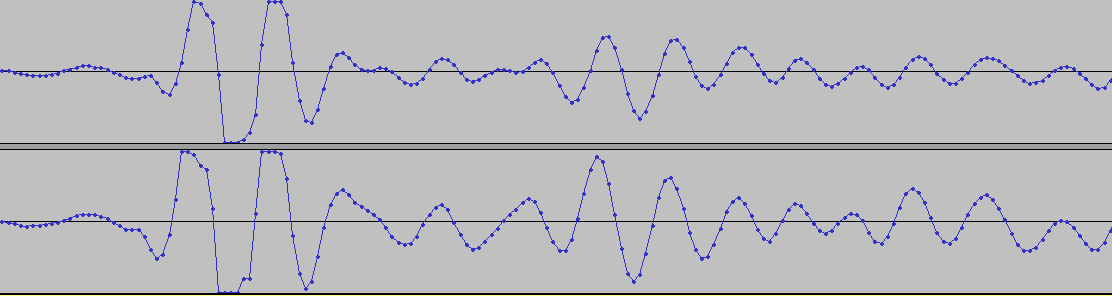
\includegraphics[width=\textwidth]{resources/img/dos_a_dos.png}
\caption{une capture d'un signal quelconque dans audacity}
\end{figure}

On remarque qu'il y a 2 signaux, ce sont les deux pistes de l'enregistrement audio. Celle du haut correspond au canal gauche, et celle du bas au canal droit.

Chaque point bleu représente un échantillon.


%\end{document}